
\chapter{Coordination Avoidance for Database Constraints}
\label{c.constraints}

Thus far, we have considered semantics expressed in terms of isolation
models and application programming patterns such as indexing. Both of
these specifications were relatively low-level. The first relied on
admissible read-write interleavings of transactions. The latter relied
on a bespoke isolation level that we introduced to exactly capture the
semantics of several existing scenarios that arise in databases and applications. In this chapter, we raise
the level of abstraction further and consider the use of
\textit{constraints}, or arbitrary user-defined predicates over
database state. We focus on constraints found in contemporary SQL and
Ruby on Rails applications.

As we discuss, these constraints are found in many database-backed
applications today. The constraints are not necessarily a full
specification of program correctness yet are frequently found in
modern applications (and are typically enforced by coordination). As candidates
for study, we draw upon popular constraints found in languages like
SQL as well as a range of constraints found in open source
applications, which we subsequently analyze for \iconfluence. As
before, we find that many are \iconfluent and provide
coordination-avoiding implementations of each.

\section{\IConfluence of SQL Constraints}
\label{sec:bcc-practice}
\label{sec:merge}

We begin our study of practical constraints by considering several
features of SQL, ending with abstract data types. We will apply these
results to full applications in Section~\ref{sec:evaluation}.

In this section, we focus on providing intuition and informal
explanations of our \iconfluence analysis. Interested readers can find
a more formal analysis in Section~\ref{sec:ic-constraints}.
including discussion of invariants not presented here. For convenience,
we reference specific proofs from Section~\ref{sec:ic-constraints} inline.


\begin{table}
\definecolor{yesgray}{gray}{0.92}
\begin{center}
\small
\begin{tabular}{|l|l|c|c|}
\hline
\textbf{Invariant} & \textbf{Operation} & \iconfluent? & Proof \#\\\hline

\rowcolor{yesgray}
Attribute Equality & Any & Yes &1\\
\rowcolor{yesgray}
Attribute Inequality & Any & Yes&2 \\
Uniqueness & Choose specific value & No&3\\
\rowcolor{yesgray}
Uniqueness & Choose some value & Yes&4\\
\texttt{AUTO\_INCREMENT} & Insert & No&5\\
\rowcolor{yesgray}
Foreign Key & Insert & Yes&6\\
Foreign Key & Delete & No&7\\
\rowcolor{yesgray}
Foreign Key & Cascading Delete & Yes&8\\
\rowcolor{yesgray}
Secondary Indexing & Update & Yes &9\\
\rowcolor{yesgray}
Materialized Views & Update & Yes &10\\\hline\hline
\rowcolor{yesgray}
> & Increment [Counter] & Yes &11 \\
< & Increment [Counter] & No &12\\
> & Decrement [Counter] & No &13\\
\rowcolor{yesgray}
< & Decrement [Counter] & Yes &14\\
\rowcolor{yesgray}
\texttt{[NOT] CONTAINS} & Any [Set, List, Map] & Yes &15, 16\\ 
\texttt{SIZE=} & Mutation [Set, List, Map] & No &17\\ \hline
\end{tabular}
\end{center}\vspace{-.5em}
\caption{Example SQL (top) and ADT \iconfluence along with
  references to formal proofs in Section~\ref{sec:ic-constraints}.}
\label{table:invariants}
\end{table}

\subsection{\IConfluence for SQL Relations}

We begin by considering several constraints found in SQL.

\minihead{Equality} As a warm-up, what if an application wants to
prevent a particular value from appearing in a database? For example,
our payroll application from Section~\ref{sec:motivation} might
require that every user have a last name, marking the \texttt{LNAME}
column with a \texttt{NOT NULL} constraint. While not particularly
exciting, we can apply \iconfluence analysis to insertions and updates
of databases with (in-)equality constraints (Claims 1, 2 in
Section~\ref{sec:ic-constraints}). Per-record inequality invariants are
\iconfluent, which we can show by contradiction: assume two database
states $S_1$ and $S_2$ are each $I$-$T$-reachable under per-record
in-equality invariant $I_e$ but that $I_e(S_1 \sqcup S_2)$ is
false. Then there must be a $r \in S_1 \sqcup S_2$ that violates $I_e$
(i.e., $r$ has the forbidden value). $r$ must appear in $S_1$, $S_2$,
or both. But, that would imply that one of $S_1$ or $S_2$ is not
$I$-valid under $I_e$, a contradiction.

\minihead{Uniqueness} We can also consider common uniqueness
invariants (e.g., \texttt{PRIMARY KEY} and \texttt{UNIQUE}
constraints). For example, in our payroll example, we wanted user IDs
to be unique. In fact, our earlier discussion in
Section~\ref{sec:motivation} already provided a counterexample showing
that arbitrary insertion of users is not \iconfluent under these
invariants: $\{$Stan:5$\}$ and $\{$Mary:5$\}$ are both
$I$-$T$-reachable states (Section~\ref{sec:ic-defs}) that can be
created by a sequence of insertions (starting at $S_0=\{\}$), but
their merge---$\{$Stan:5, Mary:5$\}$---is not $I$-valid. Therefore,
uniqueness is not \iconfluent for inserts of unique values (Claim
3). However, reads and deletions are both \iconfluent under uniqueness
invariants: reading and removing items cannot introduce duplicates.

Can the database safely \textit{choose} unique values on behalf of
users (e.g., assign a new user an ID)? In this case, we can achieve
uniqueness without coordination---as long as we have a notion of
replica membership (e.g., server or replica IDs). The difference is
subtle (``grant this record this specific, unique ID'' versus ``grant
this record some unique ID''), but, in a system model
with membership (as is practical in many contexts), is powerful. If
replicas assign unique IDs within their respective portion of the ID
namespace, then merging locally valid states will also be globally
valid (Claim 4).

\minihead{Foreign Keys} We can consider more complex invariants, such
as foreign key constraints. In our payroll example, each employee
belongs to a department, so the application could specify a constraint
via a schema declaration to capture this relationship (e.g.,
\texttt{EMP.D\_ID FOREIGN KEY REFERENCES DEPT.ID}).

Are foreign key constraints maintainable without coordination? Again,
the answer depends on the actions of transactions modifying the data
governed by the invariant. Insertions under foreign key constraints
\textit{are} \iconfluent (Claim 6). To show this, we again attempt to find two
$I$-$T$-reachable states that, when merged, result in invalid
state. Under foreign key constraints, an invalid state will contain a
record with a ``dangling pointer''---a record missing a corresponding
record on the opposite side of the association. If we assume there
exists some invalid state $S_1 \sqcup S_2$ containing a record $r$
with an invalid foreign key to record $f$, but $S_1$ and $S_2$ are
both valid, then $r$ must appear in $S_1$, $S_2$, or both. But, since
$S_1$ and $S_2$ are both valid, $r$ must have a corresponding foreign
key record ($f$) that ``disappeared'' during merge. Merge (in the
current model) does not remove versions, so this is impossible.

From the perspective of \iconfluence analysis, foreign key constraints
concern the \textit{visibility} of related updates: if individual
database states maintain referential integrity, a non-destructive
merge function such as set union cannot cause tuples to ``disappear''
and compromise the constraint. This also explains why models such as
read committed~\cite{adya} and read
atomic~\cite{adya} isolation as well as causal
consistency~\cite{hat-vldb} are also achievable without coordination:
simply restricting the visibility of updates in a given transaction's
read set does not require coordination between concurrent operations.

Deletions and modifications under foreign key constraints are more
challenging. Arbitrary deletion of records is unsafe: a user might be
added to a department that was concurrently deleted (Claim
7). However, performing cascading deletions (e.g., SQL \texttt{DELETE
  CASCADE}), where the deletion of a record also deletes \textit{all}
matching records on the opposite end of the association, is
\iconfluent under foreign key constraints (Claim 8). We can generalize
this discussion to updates (and cascading updates).

\minihead{Materialized Views} Applications often pre-compute results
to speed query performance via a materialized view~\cite{tamer-book}
(e.g., \texttt{UNREAD\_CNT} as \texttt{SELECT}\texttt{
}\texttt{COUNT(*)}\texttt{ }\texttt{FROM}\texttt{
}\texttt{emails}\texttt{ }\texttt{WHERE}\texttt{ }\texttt{read\_date =
  NULL}). We can consider a class of invariants that specify that
materialized views reflect primary data; when a transaction (or merge
invocation) modifies data, any relevant materialized views should be
updated as well. This requires installing updates at the same time as
the changes to the primary data are installed (a problem related to
maintaining foreign key constraints). However, given that a view
only reflects primary data, there are no ``conflicts.'' Thus,
materialized view maintenance updates are \iconfluent (Claim 10).

\subsection{\IConfluence for SQL Data Types}

So far, we have considered databases that store growing sets of
immutable versions. We have used this model to analyze several useful
constraints, but, in practice, databases do not (often) provide these
semantics, leading to a variety of interesting anomalies. For example,
if we implement a user's account balance using a ``last writer wins''
merge policy~\cite{crdt}, then performing two concurrent withdrawal
transactions might result in a database state reflecting only one
transaction (a classic example of the Lost Update
anomaly)~\cite{adya,hat-vldb}. To avoid variants of these
anomalies, many optimistic, coordination-free database designs have
proposed the use of \textit{abstract data types} (ADTs), providing
merge functions for a variety of uses such as counters, sets, and
maps~\cite{crdt,atomictransactions,weihl-thesis,blooml} that ensure
that all updates are reflected in final database state. For example, a
database can represent a simple counter ADT by recording the number of
times each transaction performs an \texttt{increment} operation on the
counter~\cite{crdt}.

\Iconfluence analysis is also applicable to these ADTs and their
associated invariants. For example, a row-level ``greater-than''
(\texttt{>}) threshold invariant is \iconfluent for counter
\texttt{increment} and \texttt{assign} ($\gets$) but not
\texttt{decrement} (Claims 11, 13), while a row-level ``less-than''
(\texttt{<}) threshold invariant is \iconfluent for counter
\texttt{decrement} and \texttt{assign} but not \texttt{increment}
(Claims 12, 14). This means that, in our payroll example, we can
provide \cfree support for concurrent salary increments but not
concurrent salary decrements. ADTs (including lists, sets, and maps)
can be combined with standard relational constraints like materialized
view maintenance (e.g., the ``total salary'' row should contain the
sum of employee salaries in the \texttt{employee} table).  This
analysis presumes user program explicitly use ADTs, and, as with our
generic set-union merge, \iconfluence ADT analysis requires a
specification of the ADT merge behavior (Section~\ref{sec:ic-constraints}
provides several examples).

\subsection{SQL Discussion and Limitations}

We have analyzed a number of combinations of invariants and operations
(shown in Table~\ref{table:invariants}). These results are by no
means comprehensive, but they are expressive for many applications
(Section~\ref{sec:evaluation}). In this section, we discuss lessons from this
classification process.

\minihead{Analysis mechanisms} We have manually analyzed particular
invariant and constraint combinations, demonstrating each to be
\iconfluent or not. To study actual SQL-based applications, we can
apply these labels via simple static analysis. Specifically, given
invariants (e.g., captured via SQL DDL) and transactions (e.g.,
expressed as stored procedures), we can examine each invariant and
each operation within each transaction and identify pairs that we have
labeled as \iconfluent or non-\iconfluent. Any pairs labeled as
\iconfluent can be marked as safe, while, for soundness (but not
completeness), any unrecognized operations or invariants can be
flagged as potentially non-\iconfluent. Despite its simplicity (both
conceptually and in terms of implementation), this technique---coupled
with the results of Table~\ref{table:invariants}---is sufficiently
powerful to automatically characterize the I-confluence of the
applications we consider in Section~\ref{sec:evaluation} when
expressed in SQL (with support for multi-row aggregates like Invariant
8 in Table~\ref{table:tpcc-invariants}).

By growing our recognized list of \iconfluent pairs on an as-needed
basis (via manual analysis of the pair), the above technique has
proven useful---due in large part to the common re-use of invariants
like foreign key constraints. However, one could use more complex
forms of program analysis. For example, one might analyze the
\iconfluence of \textit{arbitrary} invariants, leaving the task of
proving or disproving \iconfluence to an automated model checker or
SMT solver. While \iconfluence---like monotonicity and commutativity
(Chapter~\ref{c.relatedwork})---is undecidable for arbitrary
programs, others have recently shown this alternative approach (e.g.,
in commutativity analysis~\cite{kohler-commutativity,redblue-new} and
in invariant generation for view serializable
transactions~\cite{homeostasis}) to be fruitful for restricted
languages. We view language design and more automated analysis as an
interesting area for future work (Section~\ref{sec:c-futurework}).

\minihead{Recency and session support} Our proposed invariants are
declarative, but a class of useful semantics---recency, or real-time
guarantees on reads and writes---describe properties of operations
(i.e., they pertain to transaction execution rather than the state(s)
of the database). For example, users often wish to read data that is
up-to-date as of a given point in time (e.g., ``read
latest''~\cite{pnuts} or linearizable~\cite{gilbert-cap}
semantics). While traditional isolation models do not directly address
these recency guarantees~\cite{adya}, they are often important to
programmers. Are these models \iconfluent? We can attempt to simulate
recency guarantees in \iconfluence analysis by logging the result of
all reads and any writes with a timestamp and requiring that all
logged timestamps respect their recency guarantees (thus treating
recency guarantees as invariants over recorded read/write execution
traces). However, this is a somewhat pointless exercise: it is well
known (and we have already discussed) that recency guarantees are
unachievable with transactional
availability~\cite{hat-vldb,gilbert-cap,davidson-survey}. Thus, if
application reads face these requirements, coordination is
required. Indeed, when application ''consistency'' means ``recency,''
systems cannot circumvent speed-of-light delays.

If users wish to ``read their writes'' or desire stronger ``session''
guarantees~\cite{bayou} (e.g., maintaining recency on a per-user or
per-session basis), they must maintain affinity or
``stickiness''~\cite{hat-vldb} with a given (set of) replicas. These
guarantees are also expressible in the \iconfluence model and do
not require coordination between different users' or sessions'
transactions.


\section{More Formal \IConfluence Analysis of SQL Constraints}
\label{sec:ic-constraints}

In this section, we more formally demonstrate the \iconfluence of
invariants and operations discussed in Section~\ref{sec:merge}. Our
goals in this section are two-fold. First, we have found the
experience of formally proving \iconfluence to be instructive in
understanding these combinations (beyond less formal arguments made in
the body text for brevity and intuition). Second, we have found
\iconfluence proofs to take on two general structure typically take
one of two forms:

\begin{itemize}

\item To show a set of transactions are not \iconfluent with respect to an invariant $I$, we use proof by counterexample: we present two $I$-$T$-reachable states with a common ancestor that, when merged, are not $I$-valid. 

\item To show a set of transactions are \iconfluent with respect to an
  invariant $I$, we use proof by contradiction: we show that, if a
  state $S$ is not $I$-valid, merging two $I$-$T$-reachable states
  $S_1$ and $S_2$ with a common ancestor state to produce $S$ implies
  either one or both of $S_1$ or $S_2$ must not be $I$-valid.

\end{itemize}

These results are not exhaustive, and there are literally infinite combinations of invariants and operations to consider. Rather, the seventeen examples below serve as a demonstration of what can be accomplished via \iconfluence analysis.

Notably, the negative results below use fairly simple histories
consisting of a single transaction divergence. Nevertheless, we
decided to preserve the more general formulation of \iconfluence
(accounting for arbitrary $I$-$T$-reachable states) to account for
more pathological (perhaps less realistic, or, if these results are
any indication, less commonly encountered) behaviors that only arise
during more complex divergence patterns.

We introduce additional formalism as necessary. To start, unless
otherwise specified, we use the set union merge operator. We denote
version $i$ of item $x$ as $x_i$ and a write of version $x_i$ with
value $v$ as $w(x_i=v)$. For now, we assume each version has an
integer value.

\begin{claim}[Writes are \iconfluent with respect to per-item equality constraints]
\label{claim:eq-proof}
Assume writes are not \iconfluent with respect to some per-item equality constraint $i=c$, where $i$ is an item and $c$ is a constant. By definition, there must exist two $I$-$T$-reachable states $S_1$ and $S_2$ with common ancestor state such that $I(S_1) \rightarrow true$ and $I(S_2) \rightarrow true$ but $I(S_1 \sqcup S_2) \rightarrow false$; therefore, there exists a version $i_n$ in $S_1 \sqcup S_2$ such that $i_n \neq c$, and, under set union, $i_n \in S_1$, $i_n \in S_2$, or both. However, this would imply that $I(S_1) \rightarrow false$ or $I(S_2) \rightarrow false$ (or both), a contradiction.
\end{claim} 

\begin{claim}[Writes are \iconfluent with respect to per-item inequality constraints] \label{claim:neq} The proof follows almost identically to the proof of Claim~\ref{claim:eq-proof}, but for an invariant of the form $i\neq c$.  \end{claim}

\begin{claim}[Writing arbitrary values is not \iconfluent with respect to multi-item uniqueness constraints]
\label{claim:sunique}
Consider the following transactions:
\begin{align*}
T_{1u}&\coloneqq w(x_a=v);~commit\\
T_{2u}&\coloneqq w(x_b=v);~commit
\end{align*}
and uniqueness constraint on records:
$$I_u(D) = \{\textrm{values of versions in D are unique}\}$$
Now, an empty database trivially does not violate uniqueness constraints ($I_u(D_s=\{\})\rightarrow true$), and adding individual versions to the separate empty databases is also valid:
\begin{align*}
T_{1u}(\{\})&=\{x_a=v\},~I_u(\{x_a=v\}) \rightarrow true\\
T_{2u}(\{\})&=\{x_b=v\},~I_u(\{x_b=v\}) \rightarrow true
\end{align*}
However, merging these states results in invalid state:
$$I_u(\{x_a=v\}\sqcup \{x_b=v\} = \{x_a=v, x_b=v\}) \rightarrow false$$
Therefore, $\{T_{1u}, T_{2u}\}$ is not \iconfluent under $I_s$.
\end{claim} 

For the next proof, we consider a model as suggested in
Section~\ref{sec:bcc-practice} where replicas are able to generate
unique (but not arbitrary (!)) IDs (in the main text, we suggested the
use of a replica ID and sequence number). In the following proof, to
account for this non-deterministic choice of unique ID, we introduce a
special $nonce()$ function and require that, $nonce()$ return unique
values for each replica; this can be achieved by assigning each replica a
unique ID and implementing nonce by returning the ID along with a local sequence number. That is, $\sqcup$ is not defined for replicas
on which independent invocations of $nonce()$ return the same value.

\begin{claim}[Assigning values by $nonce()$ is \iconfluent with respect to multi-item uniqueness constraints]
\label{claim:nunique}

Assume that assigning values by $nonce()$ is not \iconfluent with respect to some multi-item uniqueness invariant:
$$I(D) = \forall c \in dom(D), \{|\{x \in D \mid x = c\}| \leq 1 \}$$
By definition, there must exist two $I$-$T$-reachable states with a common ancestor reached by executing nonce-generating transactions (of the form $T_i=[w(x_i = nonce())]$), $S_1$ and $S_2$ such that $I(S_1) \rightarrow true$ and $I(S_2) \rightarrow true$ but $I(S_1 \sqcup S_2) \rightarrow false$.

Therefore, there exist two versions $i_a, i_b$ in $S_1 \sqcup S_2$ such that $i_a$ and $i_b$ (both generated by $nonce()$) are equal in value. Under set union, this means $i_a \in S_1$ and $i_b \in S_2$ ($i_a$ and $i_b$ both cannot appear in $S_1$ or $S_2$ since it would violate those states' $I$-validity). Because replica states grow monotonically under set merge and $S_1$ and $S_2$ differ, they must be different replicas. But $nonce()$ cannot generate the same values on different replicas, a contradiction. \end{claim}

\begin{claim}[Writing arbitrary values are not \iconfluent with respect to sequentiality constraints]
\label{claim:nseq-insert}
Consider the following transactions:
\begin{align*}
T_{1s}&\coloneqq w(x_a=1);~commit\\
T_{2s}&\coloneqq w(x_b=3);~commit
\end{align*}
and the sequentiality constraint on records:
$$I_s(D) =\{max(r\in D)-min(r\in D) = |D|+1\} \vee \{|D|=0\}$$
Now, $I_s$ holds over the empty database ($I_s(\{\}) \rightarrow true$), while inserting sequential new records into independent, empty replicas is also valid:
\begin{align*}
T_{1s}(\{\})&=\{x_a=1\},~I_u(\{x_a=1\}) \rightarrow true\\
T_{2s}(\{\})&=\{x_b=3\},~I_u(\{x_b=3\}) \rightarrow true
\end{align*}
However, merging these states results in invalid state:
$$I_s(\{x_a=1\}\sqcup \{x_b=3\} = \{x_a=1, x_b=3\}) \rightarrow false$$
Therefore, $\{T_{1s}, T_{2s}\}$ is not \iconfluent under $I_s$.
\end{claim}

To discuss foreign key constraints, we need some way to \textit{refer}
to other records within the database. There are a number of ways of
formalizing this. Here, refer to a field $f$ within a given version
$x_i$ as $x_i.f$. In the following discussion, recall that
\iconfluence analysis is performed on fully replicated sets of
data. While there is considerable \textit{implementation} complexity
involved in actually performing multi-partition foreign key constraint
maintenance (and indexing; as in RAMP) this is not germane to our
model. As a simple strawman solution, we can defer all calculation of
tombstoned records until writes have quiesced, guaranteeing
convergence. As a slightly more advanced strawman, we can calculate
tombstoned records according to a global watermark of writes that is
advanced via background consensus.

\begin{claim}[Insertion is \iconfluent with respect to foreign key constraints]
\label{claim:fk-insert}
  Assume that inserting new records is not \iconfluent with respect to some foreign key constraint $I(D) = \{\forall r_f \in D$ such that $r_f.g \neq null$, $\exists r_t \in D$ such that $r_f.g = r_t.h\}$ (there exists a foreign key reference between fields $g$ and $h$). By definition, there must exist two $I$-$T$-reachable states $S_1$ and $S_2$ with a common ancestor reachable by executing transactions performing insertions such that $I(S_1) \rightarrow true$ and $I(S_2) \rightarrow true$ but $I(S_1 \sqcup S_2) \rightarrow false$; therefore, there exists some version $r_1 \in S_1 \sqcup S_2$ such that $r_1.g \neq null$ but $\nexists r_2 \in S_1 \sqcup S_2$ such that $r_1.g = r_2.h$. Under set union, $r_1$ must appear in either $S_1$ or $S_2$ (or both), and, for each set of versions in which it appears, because $S_1$ and $S_2$ are both $I$-valid, they must contain an $r_3$ such that $r_1.f = r_3.h$. But, under set union, $r_3.h$ should also appear in $S_1 \sqcup S_2$, a contradiction.
\end{claim}

For simplicity, in the following proof, we assume that deleted elements remain deleted under merge. In practice, this can be accomplished by tombstoning records and, if required, using counters to record the number of deletions and additions~\cite{crdt}. We represent a deleted version $x_d$ by $\neg x_b$.

\begin{claim}[Concurrent deletion and insertion is not \iconfluent with respect to foreign key constraints]
\label{claim:fk-delete}
 Consider the following transactions:
\begin{align*}
T_{1f}&\coloneqq w(x_a.g=1);~commit\\
T_{2f}&\coloneqq delete(x_b);~commit
\end{align*}
and the foreign key constraint:
$$I_f(D) = \{\forall r_f \in D, r_f.g \neq null,~\exists r_t \in D \suchthat \neg r_t \notin D \mathand r_f.g = r_t.h\}$$
Foreign key constraints hold over the initial database $S_i=\{x_b.h=1\}$ ($I_u(S_i) \rightarrow true$) and on independent execution of $T_a$ and $T_b$:
\begin{align*}
T_{1f}(\{x_b.h=1\})&=\{x_a.g=1, x_b.h=1\},~I_f(\{x_a=1\}) \rightarrow true\\
T_{2f}(\{x_b.h=1\})&=\{x_b.h=1, \neg {x_b}\}~I_f(\{x_b.h=1, \neg {x_b}\}) \rightarrow true
\end{align*}
However, merging these states results in invalid state: 
$$I_f(\{x_a.g=1\}\sqcup \{x_b.h=1, \neg {x_b}\}) \rightarrow false$$
Therefore, $\{T_{1f}, T_{2f}\}$ is not \iconfluent under $I_f$.\end{claim}

We denote a cascading delete of all records that reference field $f$ with value $v$ ($v$ a constant) as $cascade(f=v)$.

\begin{claim}[Cascading deletion and insertion are \iconfluent with respect to foreign key constraints]
\label{claim:fk-cascade}
Assume that cascading deletion and insertion of new records are not \iconfluent with respect to some foreign key constraint $I(D) = \{\forall r_f \in D$ such that $r_f.g \neq null$, $\exists r_t \in D$ such that $r_f.g = r_t.h$ if $cascade(h=r_f.g \neq v)\}$ (there exists a foreign key reference between fields $g$ and $h$ and the corresponding value for field $h$ has not been deleted-by-cascade). By definition, there must exist two $I$-$T$-reachable states $S_1$ and $S_2$ with common ancestor reachable by performing insertions such that $I(S_1) \rightarrow true$ and $I(S_2) \rightarrow true$ but $I(S_1 \sqcup S_2) \rightarrow false$; therefore, there exists some version $r_1 \in S_1 \sqcup S_2$ such that $r_1.f \neq null$ but $\nexists r_2 \in S_1 \sqcup S_2$ such that $r_1.g = r_2.h$. From the proof of Claim~\ref{claim:fk-insert}, we know that insertion is \iconfluent, so the absence of $r_2$ must be due to some cascading deletion. Under set union, $r_1$ must appear in exactly one of $S_1$ or $S_2$ (if $r_1$ appeared in both, there would be no deletion, a contradiction since we know insertion is \iconfluent). For the state $S_j$ in which $r_1$ does not appear (either $S_1$ or $S_2$), $S_j$ must include $cascade(h=r_1.g)$. But, if $cascade(h=r_1.g) \in S_j$, $cascade(h=r_1.g)$ must also be in $S_i \sqcup S_j$, a contradiction and so $S_i \sqcup S_j \rightarrow true$, a contradiction.
\end{claim}

We define a ``consistent'' secondary index invariant as requiring that, when a record is visible, its secondary index entry should also be visible. This is similar to the guarantees provided by Read Atomic isolation~\cite{ramp-sigmod14}. For simplicity, in the following proof, we only consider updates to a single indexed attribute $attr$, but the proof is easily generalizable to multiple index entries, insertions, and deletion via tombstones. We use last-writer wins for index entries.

\begin{claim}[Updates are \iconfluent with respect to consistent secondary indexing] \label{claim:indexing}
  Assume that updates to records are not \iconfluent with respect a secondary index constraint on attribute $attr$:

\noindent $I(D) = \{\forall r_f \in D$ such that $r_f.attr \neq null$ and $f$ is the highest version of $r\in D$, $\exists r_{idx} \in D$ such that $r_f \in r_{idx}.entries$ (all entries with non-null $attr$ are reflected in the secondary index entry for $attr$).

  Represent an update to record $r_x$ as $\{w(r_x)$ and, if $r_x.attr \neq null$, also $r_{idx}.entries.add(r_x)$, else $r_{idx}.entries.delete(r_x)\}$.

  By definition, there must exist two $I$-$T$-reachable states $S_1$ and $S_2$ with common ancestors reachable by performing insertions $S_1$ and $S_2$ such that $I(S_1) \rightarrow true$ and $I(S_2) \rightarrow true$ but $I(S_1 \sqcup S_2) \rightarrow false$; therefore, there exists some version $r_1 \in S_1 \sqcup S_2$ such that $r_1.attr \neq null$ but $\nexists r_{idx} \in S_1 \sqcup S_2$ or $\exists r_{idx} \in S_1 \sqcup S_2$ but $r_1 \notin r_{idx}.entries$. In the former case, $r_{idx} \notin S_1$ or $S_2$, but $r_1 \in S_1$ or $r_1 \in S_2$, a contradiction. The latter case also produces a contradiction: if $r_1 \in S_1$ or $r_1 \in S_2$, it must appear in $r_{idx}$, a contradiction.  \end{claim}

In our formalism, we can treat materialized views as functions over database state $f(D) \rightarrow c$.

\begin{claim}[Updates are \iconfluent with respect to materialized view maintenance] The proof is relatively straightforward if we treat the materialized view record(s) $r$ as having a foreign key relationship to any records in the domain of the function (as in the proof of Claim~\ref{claim:fk-cascade} and recompute the function on update, cascading delete, and $\sqcup$.\end{claim}

For our proofs over counter ADTs, we represent increments of a counter $c$ by $inc_i(c)$, where $i$ is a distinct invocation, decrements of $c$ by $dec_i(c)$, and the value of $c$ in database $D$ as $val(c, D) = |\{j \mid inc_j(c) \in D\}| - |\{k \mid dec_k(c) \in D\}|$.

\begin{claim}[Counter ADT increments are \iconfluent with respect to greater-than constraints] \label{claim:ge-inc-adt}
Assume increments are not \iconfluent with respect to some per-counter greater-than constraint $I(D)=val(c, D) < k$, where $k$ is a constant. By definition, there must exist two $I$-$T$-reachable states $S_1$ and $S_2$ with common ancestor reachable by executing write transactions such that $I(S_1) \rightarrow true$ and $I(S_2) \rightarrow true$ but $I(S_1 \sqcup S_2) \rightarrow false$; therefore, $val(c, S_1 \sqcup S_2) \leq k$. However, this implies that $val(c, S_1) \leq k)$, $val(c, S_2$, or both, a contradiction.  \end{claim}

\begin{claim}[Counter ADT increments are not \iconfluent with respect to less-than constraints]
\label{claim:le-inc-adt}
Consider the following transactions:
\begin{align*}
T_{1i}&\coloneqq inc_1(c);~commit\\
T_{2i}&\coloneqq inc_2(c);~commit
\end{align*}
and the less-than inequality constraint:
$$I_i(D) = \{val(c, D) < 2\}$$
$I_i$ holds over the empty database state ($I_i(\{\}) \rightarrow true$) and when $T_a$ and $T_b$ are independently executed:
\begin{align*}
T_{1i}(\{\})&=\{inc_1(c)=1\},~I_i(\{inc_1(c)=1\}) \rightarrow true\\
T_{2i}(\{\})&=\{inc_2(c)\},~I_i(\{inc_2(c)\}) \rightarrow true
\end{align*}
However, merging these states results in invalid state:
$$I_u(\{inc_1(c)\}\sqcup \{inc_2(c)\}) \rightarrow false$$
Therefore, $\{T_{1i}, T_{2i}\}$ is not \iconfluent under $I_u$.
\end{claim}

\begin{claim}[Counter ADT decrements are not \iconfluent with respect to greater-than constraints] The proof is similar to the proof of Claim~\ref{claim:le-inc-adt}; substitute $dec$ for $inc$ and choose $I_i(D) = \{val(c,D) > -2\}$.  \end{claim}

\begin{claim}[Counter ADT decrements are \iconfluent with respect to less-than constraints] \label{claim:le-inc-adt} Unsurprisingly, the proof is almost identical to the proof of Claim~\ref{claim:ge-inc-adt}, but with $<$ instead of $>$ and $dec$ instead of $inc$. \end{claim}

We provide proofs for ADT lists; the remainder are remarkably similar. Our implementation of ADT lists in these proofs uses a lexicographic sorting of values to determine list order. Transactions add a version $v$ to list $l$ via $add(v,l)$ and remove it via $del(v,l)$ (where an item is considered contained in the list if it has been added more times than it has been deleted) and access the length of $l$ in database $D$ via $size(l) = |\{k \mid add(k, l) \in D\}|- |\{m \mid del(m, l) \in D\}|$ (note that $size$ of a non-existent list is zero).

\begin{claim}[Modifying a list ADT is \iconfluent with respect to containment constraints]
  Assume ADT list modifications are not \iconfluent with respect to some equality constraint $I(D)=\{add(k, l) \in D \wedge del(k, l) \notin D \}$ for some constant $k$. By definition, there must exist two $I$-$T$-reachable states $S_1$ and $S_2$ with common ancestor reachable by list modifications such that $I(S_1) \rightarrow true$ and $I(S_2) \rightarrow true$ but $I(S_1 \sqcup S_2) \rightarrow false$; therefore, $add(k, l) \notin \{S_1 \sqcup S_2\}$ or $del(k, l) \in \{S_1 \sqcup S_2\}$. In the former case, neither $S_1$ nor $S_2$ contain $add(k,l)$ a contradiction. In the latter case, if either of $S_1$ or $S_2$ contains $del(k,l)$, it will be invalid, a contradiction.\end{claim}

\begin{claim}[Modifying a list ADT is \iconfluent with respect to non-containment constraints]
Assume ADT list modifications are not \iconfluent with respect to some non-containment constraint $I(D)=\{add(k, l) \notin D \wedge del(k, l) \in D\}$ for some constant $k$. By definition, there must exist two $I$-$T$-reachable states $S_1$ and $S_2$ with common ancestor reachable via list modifications such that $I(S_1) \rightarrow true$ and $I(S_2) \rightarrow true$ but $I(S_1 \sqcup S_2) \rightarrow false$; therefore, $add(k, l) \in \{S_1 \sqcup S_2\}$ and $del(k,l) \notin \{S_1 \sqcup S_2\}$. But this would imply that $add(k, l) \in S_1$, $add(k, l) \in S_2$, or both (while $del(k,l)$ is in neither), a contradiction.\end{claim}

\begin{claim}[Arbitrary modifications to a list ADT are not \iconfluent with respect to equality constraints on the size of the list]
Consider the following transactions:
\begin{align*}
T_{1l}&\coloneqq del(x_i, l);~add(x_a, l);~commit\\
T_{2l}&\coloneqq del(x_i, l);~add(x_b, l);~commit
\end{align*}
and the list size invariant:
$$I_l(D) = \{size(l) = 1\}$$
Now, the size invariant holds on a list of size one ($I_u(\{add(x_i, l)\}) \rightarrow true$) and on independent state modifications:
\begin{align*}
T_{1l}(\{add(x_i, l)\})&=\{add(x_i, l),~del(x_i, l),~add(x_a, l)\}\\
T_{2l}(\{add(x_i, l)\})&=\{add(x_i, l),~del(x_i, l),~add(x_b,1)\}
\end{align*}
However, merging these states result in an invalid state:
\begin{align*}
I_l(&\{add(x_i, l),~del(x_i, l),~add(x_a, l)\}\\\sqcup~&\{add(x_i, l),~del(x_i, l),~add(x_b, l)\})\rightarrow false
\end{align*}
Therefore, $\{T_{1l}, T_{2l}\}$ is not \iconfluent under $I_u$.
\end{claim}

Note that, in our above list ADT, modifying the list is \iconfluent with respect to constraints on the head and tail of the list but not intermediate elements of the list! That is, the head (resp. tail) of the merged list will be the head (tail) of one of the un-merged lists. However, the second element may come from either of the two lists.


\section{Empirical Impact: SQL-Based Constraints}
\label{sec:evaluation}

When achievable, coordination-free execution enables scalability
limited to that of available hardware. This is powerful: a
\iconfluent application can scale out without
sacrificing correctness, latency, or availability. In
Section~\ref{sec:bcc-practice}, we saw combinations of invariants
and transactions that were \iconfluent and others that were not. In this
section, we apply these combinations to the workloads of the
OLTP-Bench suite~\cite{oltpbench}, with a focus on the TPC-C
benchmark. Our focus is on the coordination required in order to
correctly execute each and the resulting, coordination-related
performance costs.

\subsection{TPC-C Invariants and Execution}
\label{sec:tpcc-invariants}

The TPC-C benchmark is the gold standard for database concurrency
control~\cite{oltpbench} both in research and in industry~\cite{tpcc},
and in recent years has been used as a yardstick for distributed
database concurrency control
performance~\cite{calvin,hstore,silo}. How much coordination does
TPC-C actually require a compliant execution?

The TPC-C workload is designed to be representative of a wholesale
supplier's transaction processing requirements. The workload has a number of
application-level correctness criteria that represent basic business
needs (e.g., order IDs must be unique) as formulated by the TPC-C
Council and which must be maintained in a compliant run. We can
interpret these well-defined ``consistency criteria'' as invariants and
subsequently use \iconfluence analysis to determine which transactions
require coordination and which do not.

Table~\ref{table:tpcc-invariants} summarizes the twelve invariants
found in TPC-C as well as their \iconfluence analysis results as
determined by Table~\ref{table:invariants}. We classify the invariants
into three broad categories: materialized view maintenance, foreign
key constraint maintenance, and unique ID assignment. As we discussed
in Section~\ref{sec:bcc-practice}, the first two categories are
\iconfluent (and therefore maintainable without coordination) because
they only regulate the \textit{visibility} of updates to multiple
records. Because these (10 of 12) invariants are \iconfluent under the
workload transactions, there exists some execution strategy that does
not use coordination. However, simply because these invariants are
\iconfluent does not mean that \textit{all} execution strategies will
scale well: for example, using locking would \textit{not} be
coordination-free.


\begin{table}[t!]
\definecolor{yesgray}{gray}{0.92}
\small
\begin{tabular}{|l|l|l|l|l|}
  \hline
  \textbf{\#} & \textbf{Informal Invariant Description} &
  \textbf{Type} & 
  \textbf{Txns} & \textbf{$\mathcal{I}$-C} \\\hline
  \rowcolor{yesgray}
  1 & {\scriptsize YTD wh sales = sum(YTD district sales)} & MV &
  P & Yes\\
  2 &  {\scriptsize Per-district order IDs are sequential} &$\mathrm{S_{ID}}$+FK  & N, D & No\\
  3 &  {\scriptsize New order IDs are sequentially assigned} & $\mathrm{S_{ID}}$  & N, D & No \\
  \rowcolor{yesgray}
  4 & {\scriptsize  Per-district, item order count = roll-up} & MV &
  N & Yes\\
  \rowcolor{yesgray}
  5 &  {\scriptsize Order carrier is set iff order is pending} & FK &
  N, D & Yes \\
  \rowcolor{yesgray}
  6 &  {\scriptsize Per-order item count = line item roll-up} & MV & N
  & Yes \\
  \rowcolor{yesgray}
  7 &  {\scriptsize Delivery date set iff carrier ID set} & FK & D & Yes \\
  \rowcolor{yesgray}
  8 &  {\scriptsize YTD wh = sum(historical wh)} & MV &
  D & Yes \\
  \rowcolor{yesgray}
  9 &  {\scriptsize YTD district = sum(historical district)} &
  MV & P & Yes \\
  \rowcolor{yesgray}
  10 &  {\scriptsize Customer balance matches expenditures} & MV & P, D & Yes \\
  \rowcolor{yesgray}
  11 &  {\scriptsize Orders reference New-Orders table}  & FK & N & Yes \\
  \rowcolor{yesgray}
  12 &  {\scriptsize Per-customer balance = cust. expenditures} & MV & P, D &
  Yes \\\hline

\end{tabular}
\caption{TPC-C Declared ``Consistency Conditions'' (3.3.2.x) and \iconfluence
  analysis results with respect to the workload transactions
  (Invariant type: MV: materialized view, $\mathbf{S_{ID}}$: sequential ID assignment, FK: foreign
  key; Transactions: N: New-Order, P: Payment, D: Delivery).}
\label{table:tpcc-invariants}
\end{table}


As one coordination-free execution strategy (which we implement in
Section~\ref{sec:evaltpcc}) that respects the foreign key and
materialized view invariants, we can use RAMP transactions from
Chapter~\ref{c.ramp}, which provide atomically visible transactional
updates across servers without relying on coordination for
correctness. As a reminder, RAMP transactions employ limited
multi-versioning and metadata to ensure that readers and writers can
always proceed concurrently: any client whose reads overlap with
another client's writes to the same item(s) can use metadata stored in
the items to fetch any ``missing'' writes from the respective
servers. A standard RAMP transaction over data items suffices to
enforce foreign key constraints, while a RAMP transaction over
commutative counters as described in~\cite{ramp-sigmod14} is sufficient to
enforce the TPC-C materialized view constraints.

Two of TPC-C's invariants are not \iconfluent with respect to the
workload transactions and therefore \textit{do} require
coordination. On a per-district basis, order IDs should be assigned
sequentially (both uniquely and sequentially, in the New-Order
transaction) and orders should be processed sequentially (in the
Delivery transaction). If the database is partitioned by warehouse (as
is standard~\cite{silo,calvin,hstore}), the former is a distributed
transaction (by default, $10\%$ of New-Order transactions span
multiple warehouses). The benchmark specification allows the latter to
be run asynchronously and in batch mode on a per-warehouse
(non-distributed) basis, so we, like others~\cite{calvin,silo}, focus
on New-Order. Including additional transactions like the read-only
Order-Status in the workload mix would increase performance due to the
transactions' lack of distributed coordination and (often
considerably) smaller read/write footprints.

\minihead{Avoiding New-Order Coordination} New-Order is not
\iconfluent with respect to the TPC-C invariants, so we can always
fall back to using serializable isolation. However, the per-district
ID assignment records (10 per warehouse) would become a point of contention,
limiting our throughput to effectively $\frac{100W}{RTT}$ for a
$W$-warehouse TPC-C benchmark with the expected $10\%$ distributed
transactions. Others~\cite{silo} (including us, in prior
work~\cite{hat-vldb}) have suggested disregarding consistency criteria
3.3.2.3 and 3.3.2.4, instead opting for unique but non-sequential ID
assignment: this allows inconsistency and violates the benchmark
compliance criteria.

During a compliant run, New-Order transactions must
coordinate. However, as discussed above, only the ID assignment
operation is non-\iconfluent; the remainder of the operations in the
transaction can execute coordination-free. With some effort, we can
avoid \textit{distributed }coordination. A na\"{\i}ve implementation might grab
a lock on the appropriate district's ``next ID'' record, perform
(possibly remote) remaining reads and writes, then release the lock at
commit time. Instead, as a more efficient solution, New-Order can
defer ID assignment until commit time by introducing a layer of
indirection. New-Order transactions can generate a temporary, unique,
but non-sequential ID (\texttt{tmpID}) and perform updates using this
ID using a RAMP transaction (which, in turn, handles the foreign key
constraints)~\cite{ramp-sigmod14}. Immediately prior to transaction
commit, the New-Order transaction can assign a ``real'' ID by
atomically incrementing the current district's local``next ID'' record
(yielding \texttt{realID}) and recording the \texttt{[tmpID, realID]}
mapping in a special ID lookup table. Any read requests for the
\texttt{ID} column of the Order, New-Order, or Order-Line tables can
be safely satisfied (transparently to the end user) by joining with
the ID lookup table on \texttt{tmpID}. In effect, the New-Order ID
assignment can use a nested atomic
transaction~\cite{atomictransactions} upon commit, and all
coordination between any two transactions is confined to a
single server.

\subsection{Evaluating TPC-C New-Order}
\label{sec:evaltpcc}


\begin{figure}
\hspace{1.5em}
\includegraphics[width=.6\columnwidth]{figs/ca_serial_legend.pdf}
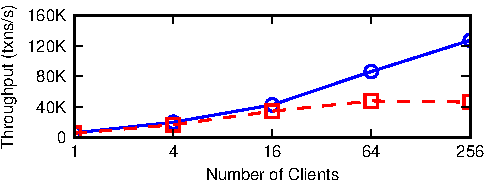
\includegraphics[width=.6\columnwidth]{figs/client_thru.pdf}
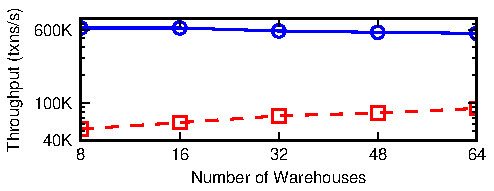
\includegraphics[width=.6\columnwidth]{figs/wh_thru.pdf}
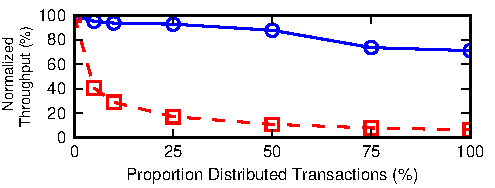
\includegraphics[width=.6\columnwidth]{figs/remote_thru.pdf}\vspace{.5em}
%\includegraphics[width=\figscale\columnwidth]{figs/wh_thru_single.pdf}
\caption{TPC-C New-Order throughput across eight servers.}
\label{fig:clients}
\end{figure}


We subsequently implemented the above execution strategy in a
distributed database prototype to quantify the overheads associated
with coordination in TPC-C New-Order. Most notably, the
coordination-avoiding query plan scales linearly to over 12.7M
transactions per second on $200$ servers while substantially
outperforming distributed two-phase locking. Our goal here is to
demonstrate---beyond the microbenchmarks of
Section~\ref{sec:motivation}---that safe but judicious use of
coordination can have meaningful positive effect on performance.

\begin{comment}
We originally ported TPC-C
New-Order to our prior RAMP transaction prototype~\cite{ramp-sigmod14} but
found that the larger transaction footprint was poorly suited for the
threading model. Each New-Order transaction generates between 13--33
reads and 13--33 writes, so switching to an event-based RPC layer with
support for batching and connection pooling delivered an approximate
factor of two improvement in throughput, while additional optimization
(e.g., more efficient indexing, fewer object allocations) delivered
another factor of two. 
\end{comment}

\minihead{Implementation and Deployment} We employ a multi-versioned
storage manager, with RAMP-Fast transactions for snapshot reads and
atomically visible writes/``merge'' (providing a variant of regular
register semantics, with writes visible to later transactions after
commit)~\cite{ramp-sigmod14} and implement the nested atomic transaction
for ID assignment as a sub-procedure inside RAMP-Fast's server-side
commit procedure (using spinlocks). We implement transactions as
stored procedures and fulfill the TPC-C ``Isolation Requirements'' by
using read and write buffering as proposed in~\cite{hat-vldb}. As is
common~\cite{calvin,abadi-vll,hstore,jones-dtxn}, we disregard
per-warehouse client limits and ``think time'' to increase load per
warehouse. In all, our base prototype architecture is similar to that
of~\cite{ramp-sigmod14}: a JVM-based partitioned, main-memory, mastered
database.

For an apples-to-apples comparison with a coordination-intensive
technique within the same system, we also implemented textbook
two-phase locking (2PL)~\cite{bernstein-book}, which provides
serializability but also requires distributed coordination. We totally
order lock requests across servers to avoid deadlock, batching lock
requests to each server and piggybacking read and write requests on
lock request RPC. As a validation of our implementation, our 2PL
prototype achieves per-warehouse (and sometimes aggregate) throughput
similar to (and often in excess of) several recent serializable
database implementations (of both 2PL and other
approaches)~\cite{calvin,abadi-vll,hstore,jones-dtxn}.

By default, we deploy our prototype on eight EC2 \texttt{cr1.8xlarge}
instances (32 cores comprising 88 Amazon Elastic Compute units, each
with 244GB RAM) in the Amazon EC2 \texttt{us-west-2} region with
non-co-located clients and one warehouse per server (recall there
are 10 ``hot'' district ID records per warehouse) and report the
average of three 120 second runs.

\minihead{Basic behavior} Figure~\ref{fig:clients} shows performance
across a variety of configurations, which we detail below. Overall,
the coordination-avoiding query plan far outperforms the serializable
execution. The coordination-avoiding query plan performs some
coordination, but, because coordination points are not distributed
(unlike 2PL), physical resources (and not coordination) are the bottleneck.

\miniheadit{Varying load} As we increase the number of clients, the
coordination-avoiding query plan throughput increases linearly, while
2PL throughput increases to $40$K transactions per second, then levels
off. As in our microbenchmarks in
Section~\ref{sec:background-cmotivation}, the former utilizes
available hardware resources (bottlenecking on CPU cycles at $640$K
transactions per second), while the latter bottlenecks on logical
contention.

\miniheadit{Physical resource consumption} To understand the overheads
of each component in the coordination-avoiding query plan, we used JVM
profiling tools to sample thread execution while running at peak
throughput, attributing time spent in functions to relevant modules
within the database implementation (where possible):

\begin{center}
\centering
\small
\setlength{\fboxsep}{4pt}
\fbox{
\begin{tabular}{l r}
\textbf{Code Path} & \textbf{Cycles}\\
Storage Manager (Insert, Update, Read) & 45.3\%\\
Stored Procedure Execution & 14.4\%\\
RPC and Networking & 13.2\%\\
Serialization & 12.6\%\\
ID Assignment Synchronization (spinlock contention) & 0.19\%\\
Other & 14.3\%\\
\end{tabular}}
\end{center}

The coordination-avoiding prototype spends a large portion of
execution in the storage manager, performing B-tree modifications and
lookups and result set creation, and in RPC/serialization. In contrast
to 2PL, the prototype spends less than $0.2\%$ of time coordinating,
in the form of waiting for locks in the New-Order ID assignment; the
(single-site) assignment is fast (a linearizable integer increment and
store, followed by a write and fence instruction on the spinlock), so
this should not be surprising. We observed large throughput penalties
due to garbage collection (GC) overheads (up to 40\%)---an unfortunate
cost of our highly compact (several thousand lines of Scala),
JVM-based implementation. However, even in this current prototype,
physical resources are the bottleneck---not coordination.

\miniheadit{Varying contention} We subsequently varied the number of
``hot,'' or contended items by increasing the number of warehouses on
each server. Unsurprisingly, 2PL benefits from a decreased
contention, rising to over $87$K transactions per second with $64$
warehouses. In contrast, our coordination-avoiding implementation is
largely unaffected (and, at $64$ warehouses, is even negatively
impacted by increased GC pressure). The coordination-avoiding query
plan is effectively agnostic to read/write contention.

\miniheadit{Varying distribution} We also varied the percentage of
distributed transactions. The coordination-avoiding query plan
incurred a $29\%$ overhead moving from no distributed transactions to
all distributed transactions due to increased serialization overheads
and less efficient batching of RPCs. However, the 2PL implementation decreased in throughput by over $90\%$ (in line
with prior results~\cite{abadi-vll,calvin}, albeit exaggerated here
due to higher contention) as more requests stalled due to coordination
with remote servers.

\minihead{Scaling out} Finally, we examined our prototype's scalability,
again deploying one warehouse per server. As Figure~\ref{fig:scaleout}
demonstrates, our prototype scales linearly, to over 12.74 million
transactions per second on 200 servers (in light of our earlier
results, and, for economic reasons, we do not run 2PL at this
scale). Per-server throughput is largely constant after 100 servers,
at which point our deployment spanned all three \texttt{us-west-2}
datacenters and experienced slightly degraded per-server performance.
While we make use of application semantics, we are unaware of
any other compliant multi-server TPC-C implementation that has
achieved greater than 500K New-Order transactions per
second~\cite{calvin,jones-dtxn,hstore,abadi-vll}.

\minihead{Summary} We present these quantitative results as a proof of
concept that executing even challenging workloads like TPC-C that
contain complex integrity constraints are not necessarily at odds with
scalability if implemented in a coordination-avoiding
manner. Distributed coordination need not be a bottleneck for all
applications, even if conflict serializable execution indicates
otherwise. Coordination avoidance ensures that physical
resources---and not logical contention---are the system bottleneck
whenever possible.

\begin{figure}
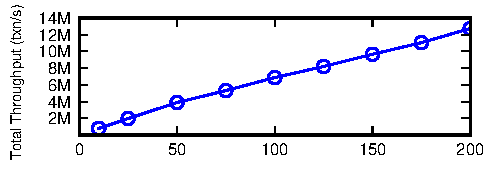
\includegraphics[width=\figscale\columnwidth]{figs/scale_thru_total.pdf}
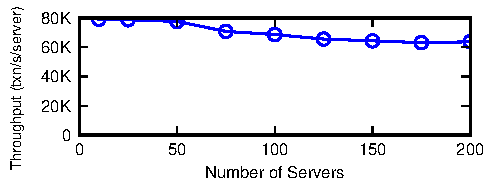
\includegraphics[width=\figscale\columnwidth]{figs/scale_thru_each.pdf}\vspace{.5em}
\caption{Coordination-avoiding New-Order scalability.}
\label{fig:scaleout}
\end{figure}

\subsection{Analyzing Additional Applications}

These results begin to quantify the effects of coordination-avoiding
concurrency control. If considering \textit{application-level}
invariants, databases only have to pay the price of coordination when
necessary. We were surprised that the ``current industry standard for
evaluating the performance of OLTP systems''~\cite{oltpbench} was so
amenable to coordination-avoiding execution---at least for compliant
execution as defined by the official TPC-C specification.

For greater variety, we also studied the workloads of the recently
assembled OLTP-Bench suite~\cite{oltpbench}, performing a similar
analysis to that of Section~\ref{sec:tpcc-invariants}. We found (and
confirmed with an author of~\cite{oltpbench}) that for nine of
fourteen remaining (non-TPC-C) OLTP-Bench applications, the workload
transactions did not involve integrity constraints (e.g., did not
modify primary key columns), one (\texttt{CH-benCHmark}) matched
TPC-C, and two specifications implied (but did not explicitly state) a
requirement for unique ID assignment (\texttt{AuctionMark}'s
\texttt{new-purchase} order completion, \texttt{SEATS}'s
\texttt{NewReservation} seat booking; achievable like TPC-C order
IDs). The remaining two benchmarks, \texttt{sibench} and
\texttt{smallbank} were specifically designed as research benchmarks
for serializable isolation. Finally, the three ``consistency
conditions'' required by the newer TPC-E benchmark are a proper subset
of the twelve conditions from TPC-C considered here (and are all
materialized counters). It is possible (even likely) that these
benchmarks are underspecified, but according to official
specifications, TPC-C contains the most coordination-intensive
invariants among all but two of the OLTP-Bench workloads.

Anecdotally, our conversations and experiences with real-world
application programmers and database developers have not identified
invariants that are radically different than those we have studied
here. A simple thought experiment identifying the invariants required
for a social networking site yields a number of invariants but none
that are particularly exotic (e.g., username uniqueness, foreign key
constraints between updates, privacy
settings~\cite{pnuts,ramp-sigmod14}). Nonetheless, we examine
additional invariants from real-world applications in the remainder of
this chapter. The results presented in this section hint at what is
possible with coordination-avoidance as well as the costs of
coordination if applications are not \iconfluent.

\section{Constraints from Open Source Applications}
\label{sec:rails-intro}

In the remainder of this chapter, we examine constraints as found in
modern, open source web applications. The rise of ``Web 2.0'' Internet
applications delivering dynamic, highly interactive user experiences
has been accompanied by a new generation of programming
frameworks~\cite{web20}. These frameworks simplify common tasks such
as content templating and presentation, request handling, and,
notably, data storage, allowing developers to focus on ``agile''
development of their applications. This trend embodies the most recent
realization of the larger vision of object-relational mapping (ORM)
systems~\cite{orm-db}, albeit at a unprecedented scale of deployment
and programmer adoption.

As a lens for understanding issues of data integrity in modern ORM
systems, we study Ruby on Rails (or, simply,
``Rails'')~\cite{rails-book,rails-computer}, a central player among
modern frameworks powering sites including (at one point)
Twitter~\cite{twitter-rails}, Airbnb~\cite{airbnb-rails},
GitHub~\cite{github-rails}, Hulu~\cite{hulu-rails},
Shopify~\cite{shopify-rails}, Groupon~\cite{groupon-rails},
SoundCloud~\cite{soundcloud-rails}, Twitch~\cite{twitch-rails},
Goodreads~\cite{goodreads-rails}, and
Zendesk~\cite{zendesk-rails}. From the perspective of database systems
research, Rails is interesting for at least two reasons. First, it
continues to be a popular means of developing responsive web
application front-end and business logic, with an active open source
community and user base. Rails recently celebrated its tenth
anniversary and enjoys considerable commercial interest, both in terms
of deployment and the availability of hosted ``cloud'' environments
such as Heroku. Thus, Rails programmers represent a large class of
consumers of database technology. Second, and perhaps more
importantly, Rails is ``opinionated
software''~\cite{dhh-opinionated}. That is, Rails embodies the strong
personal convictions of its developer community, and, in particular,
David Heinemeier Hansson (known as DHH), its creator. Rails is
particularly opinionated towards the database systems that it tasks
with data storage. To quote DHH:
\begin{quote}
``I don't \textit{want} my database to be clever! \dots I consider stored procedures and constraints vile and reckless destroyers of coherence. No, Mr. Database, you can not have my business logic. Your procedural ambitions will bear no fruit and you'll have to pry that logic from my dead, cold object-oriented hands \dots I want a single layer of cleverness: My domain model.''~\cite{dhh-clever}
\end{quote}
Thus, in several regards, this wildly successful software framework bears
an actively antagonistic relationship to database management systems,
echoing a familiar refrain of the ``NoSQL'' movement: get the database
out of the way and let the application do the work.

In this paper, we examine the implications of this impedance mismatch
between databases and modern ORM frameworks in the context of
application integrity. Rails largely ignores decades of work on native
database concurrency control solutions by providing a set of
primitives for handling application integrity that are enforced at the
application tier---building, from the underlying database system's
perspective, a \textit{feral} concurrency control system. Core to
feral concurrency control mechanisms is the use of data invariants, as
we have studied in this chapter in the context of SQL. We examine the
design and use of these feral mechanisms and evaluate their
effectiveness in practice by analyzing them and experimentally
quantifying data integrity violations in practice. Our goal is to
understand how this growing class of applications currently interacts
with database systems and how we, as a database systems community, can
positively engage with these criticisms to better serve the needs of
these developers.

We begin by surveying the state of Rails' application-tier concurrency
control primitives and examining their use in 67 open source
applications representing a variety of use cases from e-Commerce to
Customer Relationship Management and social networking. We find that,
these applications overwhelmingly use Rails' built-in support for
declarative invariants---\textit{validations} and
\textit{associations}---to protect data integrity---instead of
application-defined transactions, which are used more than 37 times less
frequently. Across the survey, we find over $9950$ uses of
application-level validations designed to ensure correctness criteria
including referential integrity, uniqueness, and adherence to common
data formats.

Given this corpus, we subsequently ask: are these feral invariants
correctly enforced? Do they work in practice? Rails may execute
validation checks in parallel, so we study the potential for data
corruption due to races if validation and update activity does not run
within a serializable transaction in the database. This is a real
concern, as many DBMS platforms use non-serializable isolation by
default and in many cases (despite labeling otherwise) do not provide
serializable isolation as an option at all.  Accordingly, we apply
\iconfluence analysis and show that, in fact, up to $86.9\%$ of Rails
validation usage by volume is actually \iconfluent and therefore safe
under concurrent execution. However, the remainder---which include
uniqueness violations under insertion and foreign key constraint
violations under deletion---are not. Therefore, we quantify the impact
of concurrency on data corruption for Rails uniqueness and foreign key
constraints under both worst-case analysis and via actual Rails
deployment. We demonstrate that, for pathological workloads,
validations reduce the severity of data corruption by orders of
magnitude but nevertheless still permit serious integrity violations.

Given these results, we return to our goal of improving the underlying
data management systems that power these applications and present
recommendations for the database research community. We expand our
study to survey several additional web frameworks and demonstrate that
many also provide a notion of feral validations, suggesting an
industry-wide trend. While the success of Rails and its ilk---despite
(or perhaps due to) their aversion to database technology---are firm
evidence of the continued impedance mismatch between object-oriented
programming and the relational model, we see considerable opportunity
in improving database systems to better serve these communities---via
more programmer- and ORM-friendly interfaces that ensure correctness
while minimizing impacts on performance and portability.

\subsection{Background and Context}
\label{sec:motivation}

As a primary focus of our study, we investigate the operational model, database use, and application primitives provided in Rails. In this section, we provide a overview of the Rails programming model and describe standard Rails deployment architectures.

\subsubsection{Rails Tenets and MVC}
\label{sec:mvc}

Rails was developed in order to maximize developer productivity. This focus is captured by two core architectural principles~\cite{rails-book}. First, Rails adopts a ``Don't Repeat Yourself'' (DRY) philosophy: ``every piece of knowledge should be expressed in just one place'' in the code. Data modeling and schema descriptions are relegated to one portion of the system, while presentation and business logic are relegated to two others. Rails attempts to minimize the amount of boilerplate code required to achieve this functionality. Second, Rails adopts a philosophy of ``Convention over Configuration,'' aiming for sensible defaults and allowing easy deployment without many---if any---modifications to configuration.

A natural corollary to the above principles is that Rails encourages an idiomatic style of programming. The Rails framework authors claim that ``somehow, [this style] just seems right'' for quickly building responsive web applications~\cite{rails-book}. The framework's success hints that its idioms are, in fact, natural to web developers.

More concretely, Rails divides application code into a three-component architecture called Model-View-Controller~\cite{gangoffour,mvc}:

\begin{itemize}
\item The \textbf{Model} acts as a basic ORM and is responsible for
  representing and storing business objects, including schemas,
  querying, and persistence functionality. For example, in a banking
  application, an account's state could be represented by a model with
  a numeric owner ID field and a numeric balance field.

\item The \textbf{View} acts as a presentation layer for application objects, including rendering into browser-ingestible HTML and/or other formats such as JSON. In our banking application, the View would be responsible for rendering the page displaying a user's account balance.

\item The \textbf{Controller} encapsulates the remainder of the application's business logic, including actual generation of queries and transformations on the Active Record models. In our banking application, we would write logic for orchestrating withdrawal and deposit operations within the Controller.
\end{itemize}

Actually building a Rails application is a matter of instantiating a collection of models and writing appropriate controller and presentation logic for each.

As we are concerned with how Rails utilizes database back-ends, we largely focus on how Rails applications interact with the Model layer. Rails natively supports a Model implementation called \texttt{Active Record}. Rails's Active Record module is an implementation of the Active Record pattern originally proposed by Martin Fowler, a prominent software design consultant~\cite{fowler-book}. Per Fowler, an Active Record is ``an object that wraps a row in a database or view, encapsulates the database access, and adds domain logic on that data'' (further references to Active Record will correspond to Rails's implementation). The first two tasks---persistence and database encapsulation---fit squarely in the realm of standard ORM design, and Rails adopts Fowler's recommendation of a one-to-one correlation between object fields and database columns (thus, each declared Active Record class is stored in a separate table in the database). The third component, domain logic, is more complicated. Each Rails model may contain a number of attributes (and must include a special primary-key-backed \texttt{id} field) as well as associated logic including data validation, associations, and other constraints. Fowler suggests that ``domain logic that isn't too complex'' is well-suited for encapsulation in an Active Record class. We will discuss these in greater depth in the next section.

\subsubsection{Databases and Deployment}
\label{sec:deployment}

This otherwise benign separation of data and logic becomes interesting when we consider how Rails servers process concurrent requests. In this section, we describe how, in standard Rails deployments, application logic may be executed concurrently and without synchronization within separate threads or processes.

In Rails, the database is---at least for basic usages---simply a place to store model state and is otherwise divorced from the application logic. All application code is run within the Ruby virtual machine (VM), and Active Record makes appropriate calls to the database in order to materialize collections of models in the VM memory as needed (as well as to persist model state). However, from the database's perspective (and per DHH's passionate declaration in Section~\ref{sec:rails-intro}), logic remains in the application layer. Active Record natively provides support for PostgreSQL, MySQL, and SQLite, with extensions for databases including Oracle and is otherwise agnostic to database choice.

Rails deployments typically resemble traditional multi-tier web architectures~\cite{alonso-web} and consist of an HTTP server such as Apache or Nginx that acts as a proxy for a pool of Ruby VMs running the Rails application stack. Depending on the Ruby VM and Rails implementation, the Rails application may or may not be multi-threaded.\footnote{Ruby was not traditionally designed for highly concurrent operations: its standard reference VM---Ruby MRI---contains (like Python's CPython) a ``Global VM Lock'' that prevents multiple OS threads from executing at a given time. While alternative VM implementations provide more concurrent behavior, until Rails 2.2 (released in November 2008), Rails embraced this behavior and was unable to process more than one request at a time (due to state shared state including database connections and logging state)~\cite{rails-threading}. In practice today, the choice of multi-process, multi-threaded, or multi-process and multi-threaded deployment depends on the actual application server architecture. For example, three popular servers---Phusion Passenger, Puma, and Unicorn ---each provide a different configuration.} Thus, when an end-user makes a HTTP request on a Rails-powered web site, the request is first accepted by a web server and passed to a Rails worker process (or thread within the process). Based on the HTTP headers and destination, Rails subsequently determines the appropriate Controller logic and runs it, including any database calls via Active Record, and renders a response via the View, which is returned to the HTTP server.

Thus, in a Rails application, the \textit{only} coordination between individual application requests occurs within the database system. Controller execution---whether in separate threads or across Ruby VMs (which may be active on different physical servers)---is entirely independent, save for the rendezvous of queries and modifications within the database tier, as triggered by Active Record operations.

The independent execution of concurrent business logic should give
serious pause to disciples of transaction processing systems. Is this
execution strategy actually safe? Thus far, we have yet to discuss any
mechanisms for maintaining correct application data, such as the use
of transactions. In fact, as we will discuss in the next section,
Rails has, over its lifetime, introduced several mechanisms for
maintaining consistency of application data. In keeping with Rails'
focus on maintaining application logic within Rails (and not within the
database), this has led to several different proposals. In the
remainder of this paper, we examine their use and whether, in fact,
they correctly maintain application data.




\subsection{Feral Mechanisms in Rails}
\label{sec:rails-cc}

As we discussed in Section~\ref{sec:deployment}, Rails services user
requests independently, with the database acting as a point
of rendezvous for concurrent operations. Given Rails's design goals of
maintaining application logic at the user level, this appears---on its
face---a somewhat cavalier proposition with respect to application
integrity. In response, Rails has developed a range of concurrency
control strategies, two of which operate external to the database, at
the application level, which we term \textit{feral concurrency
  control} mechanisms.

In this section, we outline four major mechanisms for guarding against
integrity violations under concurrent execution in Rails. We
subsequently begin our study of 67 open source applications to
determine which of these mechanisms are used in practice. In the following
section, we will determine which are sufficient to maintain
correct data---and when they are not.

\subsubsection{Rails Concurrency Control Mechanisms}

Rails contains four main mechanisms for concurrency control.

\begin{enumerate}
\item Rails provides support for \textbf{transactions}. By wrapping a
sequence of operations within a special \texttt{transaction} block,
Rails operations will execute transactionally, backed by an actual
database transaction. The database transaction either runs at the
database's configured default isolation level or, as of Rails 4.0.0, can
be configured on a per-transaction
basis~\cite{code-transaction-isolation}.

\item Rails provides support for both optimistic and pessimistic
  per-record \textbf{locking}. Applications invoke pessimistic locks
  on an Active Record object by calling its \texttt{lock} method,
  which invokes a \texttt{SELECT FOR UPDATE} statement in the
  database. Optimistic locking is invoked by declaring a special
  \texttt{lock\_version} field in an Active Record model. When a Rails
  process performs an update to an optimistically locked model, Active
  Record uses a transaction to atomically check whether the corresponding record's
  \texttt{lock\_version} field has changed since the process last read
  the object. If the record has not changed, Rails transactionally increments
  \texttt{lock\_version} and updates the database record; if the
  record has changed, the update fails.

\item Rails provides support for application-level
  \textbf{validations}. Each Active Record model has a set of zero or more
  validations, or boolean-valued functions, and a model instance many
  only be saved to the database if all of its declared validations
  return true. These validations ensure, for example, that particular
  fields within a record are not null or are unique
  within the database. Rails provides a number of built-in validations
  but also allows arbitrary user-defined validations (we discuss
  actual validations further in subsequent sections). The framework
  runs each declared validation sequentially and, if all succeed, the
  model state is updated in the database; this happens within a
  database-backed transaction.\footnote{The practice of wrapping
    validations in a transaction dates to the earliest public Rails
    commit (albeit, in 2004, transactions were only supported via a
    per-Ruby VM global lock~\cite{code-txn-lock}). However, as late as
    2010, updates were only partially protected by
    transactions~\cite{code-txn-update}.} The validations supported by
  Rails today include ones that are natively supported by many
  commercial databases today, as well as others.\\[-2mm]

\item Rails provides support for application-level
  \textbf{associations}. As the name suggests, ``an association is a
  connection between two Active Record models,'' effectively acting
  like a foreign key in an RDBMS. Associations can be declared on one
  or both sides of a one-to-one or one-to-many relationship, including
  transitive dependencies (via a \texttt{:through}
  annotation). Declaring an association (e.g., \texttt{:belongs\_to
    dept}) produces a special field for the associated record ID
  within the model (e.g., \texttt{dept\_id}). Coupling an association
  with an appropriate validation (e.g., \texttt{:presence}) ensures
  that the association is indeed valid (and is, via the validation,
  backed by a database transaction). Until the release of Rails 4.2 in
  December 2014, Rails did not provide native support for
  database-backed foreign key constraints. In Rails 4.2, foreign keys
  are supported via manual schema annotations declared separately from
  each model; declaring an association does not declare a
  corresponding foreign key constraint and vice-versa.
\end{enumerate}

Overall, these four mechanisms provide a range of options for
developers. The first is squarely in the realm of traditional
concurrency control. The second is, in effect, a coarse-grained
user-level implementation of single-record transactions via
database-level ``compare-and-swap'' primitives (implemented via
\texttt{SELECT FOR UPDATE}). However, the latter two---validations and
associations---operate, in effect, at the application level. Although
some validations like uniqueness validations have analogs in an RDBMS,
the semantics of these validations are entirely contained within the
Rails code. In effect, from the database's perspective, these
validations exist external to the system and are \textit{feral}
concurrency control mechanisms.

Rails's feral mechanisms---validations and associations---are a
prominent feature of the Active Record model. In contrast, neither
transactions nor locks are actually discussed in the official ``Rails
Guides,'' and, generally, are not promoted as a means of ensuring data
integrity. Instead, the Rails documentation~\cite{rails-guide} prefers
validations as they are ``are database agnostic, cannot be bypassed by
end users, and are convenient to test and maintain.'' Moreover, the
Rails documentation opines that ``database constraints and/or stored
procedures make the validation mechanisms database-dependent and can
make testing and maintenance more difficult.''  As we will show
shortly, these feral mechanisms accordingly dominate in terms of
developer popularity in real applications.

\subsubsection{Adoption in Practice}

To understand exactly how users interact with these
concurrency control mechanisms and determine which deserved more
study, we examined their usage in a portfolio of publicly available
open source applications. We find that validations and associations
are overwhelmingly the most popular forms of concurrency control.

\minihead{Application corpus} We selected 67 open source applications
built using Ruby on Rails and Active Record, representing a variety of
application domains, including eCommerce, customer relationship
management, retail point of sale, conference management, content
management, build management, project management, personal task
tracking, community management and forums, commenting, calendaring,
file sharing, Git hosting, link aggregation, crowdfunding, social
networking, and blogging. We sought projects with substantial
code-bases (average: 26,809 lines of Ruby) multiple contributors
(average: 69.1), and relative popularity (measured according to GitHub
stars) on the site. Table~\ref{table:app-summary} provides a detailed overview.

To determine the occurrences and number of models, transactions, locks, validations, and associations in Rails, we wrote a set of analysis scripts that performed a very rudimentary syntactic static analysis . We do not consider the analysis techniques here a contribution; rather, our interest is in the output of the analysis. The syntactic approach proved portable between the many versions of Rails against which each application is linked; otherwise, porting between non-backwards-compatible Rails versions was difficult and, in fact, unsupported by several of the Rails code analysis tools we considered using as alternatives. The choice to use syntax as a means of distinguishing code constructs led to some ambiguity. To compensate, we introduced custom logic to handle esoteric syntaxes that arose in particular projects (e.g., some projects extend \texttt{ActiveRecord::Base} with a separate, project-specific base class, while some validation usages vary between constructs like \texttt{:validates\_presence} and \texttt{:validates\_presence\_of}).

To determine code authorship, we used the output of git \texttt{log} and \texttt{blame} and did not attempt any sophisticated entity resolution.



\begin{landscape}
\footnotesize
\begin{longtable}{{|l}*{12}{l}{l|}}\hline
Name & Description & Authors & LoC Ruby & Commits &
 M & {\scriptsize T} & \scriptsize{PL} & \scriptsize{OL} & \scriptsize{V} &
 \scriptsize{A} & \scriptsize{Stars} &  \tiny{Githash} & \tiny{Last
   commit}\\\hline
Canvas LMS & {\scriptsize{Education}} & 132 & 309,580 & 12,853 & 161 & 46 & 12 & 1 & 354 & 837 & 1,251 & {\tiny\texttt{3fb8e69}} & {\tiny{10/16/14}}\\
OpenCongress & {\scriptsize{Congress data}} & 15 & 30,867 & 1,884 & 106 & 1 & 0 & 0 & 48 & 357 & 124 & {\tiny\texttt{850b602}} & {\tiny{02/11/13}}\\
Fedena & {\scriptsize{Education management}} & 4 & 49,297 & 1,471 & 104 & 5 & 0 & 0 & 153 & 317 & 262 & {\tiny\texttt{40cafe3}} & {\tiny{01/23/13}}\\
Discourse & {\scriptsize{Community discussion}} & 440 & 72,225 & 11,480 & 77 & 41 & 0 & 0 & 83 & 266 & 12,233 & {\tiny\texttt{1cf4a0d}} & {\tiny{10/20/14}}\\
Spree & {\scriptsize{eCommerce}} & 677 & 47,268 & 14,096 & 72 & 6 & 0 & 0 & 92 & 252 & 5,582 & {\tiny\texttt{aa34b3a}} & {\tiny{10/16/14}}\\
Sharetribe & {\scriptsize{Content management}} & 35 & 31,164 & 7,140 & 68 & 0 & 0 & 0 & 112 & 202 & 127 & {\tiny\texttt{8e0d382}} & {\tiny{10/21/14}}\\
ROR Ecommerce & {\scriptsize{eCommerce}} & 19 & 16,808 & 1,604 & 63 & 2 & 3 & 0 & 219 & 207 & 857 & {\tiny\texttt{c60a675}} & {\tiny{10/09/14}}\\
Diaspora & {\scriptsize{Social network}} & 388 & 31,726 & 14,640 & 63 & 2 & 0 & 0 & 66 & 128 & 9,571 & {\tiny\texttt{1913397}} & {\tiny{10/03/14}}\\
Redmine & {\scriptsize{Project management}} & 10 & 81,536 & 11,042 & 62 & 11 & 0 & 1 & 131 & 157 & 2,264 & {\tiny\texttt{e23d4d9}} & {\tiny{10/19/14}}\\
ChiliProject & {\scriptsize{Project management}} & 53 & 66,683 & 5,532 & 61 & 7 & 0 & 1 & 118 & 130 & 623 & {\tiny\texttt{984c9ff}} & {\tiny{08/13/13}}\\
Spot.us & {\scriptsize{Community reporting}} & 46 & 94,705 & 9,280 & 58 & 0 & 0 & 0 & 96 & 165 & 343 & {\tiny\texttt{61b65b6}} & {\tiny{12/02/13}}\\
Jobsworth & {\scriptsize{Project management}} & 46 & 24,731 & 7,890 & 55 & 10 & 0 & 0 & 86 & 225 & 478 & {\tiny\texttt{3a1f8e1}} & {\tiny{09/12/14}}\\
OpenProject & {\scriptsize{Project management}} & 63 & 84,374 & 11,185 & 49 & 8 & 1 & 3 & 136 & 227 & 371 & {\tiny\texttt{c1e66af}} & {\tiny{11/21/13}}\\
Danbooru & {\scriptsize{Image board}} & 25 & 27,857 & 3,738 & 47 & 9 & 0 & 0 & 71 & 114 & 238 & {\tiny\texttt{c082ed1}} & {\tiny{10/17/14}}\\
Salor Retail & {\scriptsize{Point of Sale}} & 26 & 18,404 & 2,259 & 44 & 0 & 0 & 0 & 81 & 309 & 24 & {\tiny\texttt{00e1839}} & {\tiny{10/07/14}}\\
Zena & {\scriptsize{Content management}} & 7 & 56,430 & 2,514 & 44 & 1 & 0 & 0 & 12 & 43 & 172 & {\tiny\texttt{79576ac}} & {\tiny{08/18/14}}\\
Skyline CMS & {\scriptsize{Content management}} & 7 & 10,404 & 894 & 40 & 5 & 0 & 0 & 28 & 89 & 127 & {\tiny\texttt{64b0932}} & {\tiny{12/09/13}}\\
Opal & {\scriptsize{Project management}} & 6 & 10,707 & 474 & 38 & 3 & 0 & 0 & 42 & 96 & 45 & {\tiny\texttt{11edf34}} & {\tiny{01/09/13}}\\
OneBody & {\scriptsize{Church portal}} & 33 & 20,398 & 3,973 & 36 & 3 & 0 & 0 & 97 & 140 & 1,041 & {\tiny\texttt{2dfbd4d}} & {\tiny{10/19/14}}\\
CommunityEngine & {\scriptsize{Social networking}} & 67 & 13,967 & 1,613 & 35 & 3 & 0 & 0 & 92 & 101 & 1,073 & {\tiny\texttt{a4d3ea2}} & {\tiny{10/16/14}}\\
Publify & {\scriptsize{Blogging}} & 93 & 16,763 & 5,067 & 35 & 7 & 0 & 0 & 33 & 50 & 1,274 & {\tiny\texttt{4acf86e}} & {\tiny{10/20/14}}\\
Comas & {\scriptsize{Conference management}} & 5 & 5,879 & 435 & 33 & 6 & 0 & 0 & 80 & 45 & 21 & {\tiny\texttt{81c25a4}} & {\tiny{09/09/14}}\\
BrowserCMS & {\scriptsize{Content management}} & 56 & 21,259 & 2,503 & 32 & 4 & 0 & 0 & 47 & 77 & 1,183 & {\tiny\texttt{d654557}} & {\tiny{09/30/14}}\\
RailsCollab & {\scriptsize{Project management}} & 25 & 8,849 & 865 & 29 & 6 & 0 & 0 & 40 & 122 & 262 & {\tiny\texttt{9f6c8c1}} & {\tiny{02/16/12}}\\
OpenGovernment & {\scriptsize{Government data}} & 15 & 9,383 & 2,231 & 28 & 4 & 0 & 0 & 22 & 141 & 160 & {\tiny\texttt{fa80204}} & {\tiny{11/21/13}}\\
Tracks & {\scriptsize{Personal productivity}} & 89 & 17,419 & 3,121 & 27 & 2 & 0 & 0 & 24 & 43 & 639 & {\tiny\texttt{eb2650c}} & {\tiny{10/02/14}}\\
GitLab & {\scriptsize{Code management}} & 671 & 39,094 & 12,266 & 24 & 15 & 0 & 0 & 131 & 114 & 14,129 & {\tiny\texttt{72abe9f}} & {\tiny{10/20/14}}\\
Brevidy & {\scriptsize{Video sharing}} & 2 & 7,608 & 6 & 24 & 1 & 0 & 0 & 74 & 56 & 167 & {\tiny\texttt{d0ddb1a}} & {\tiny{01/18/14}}\\
Insoshi & {\scriptsize{Social network}} & 16 & 121,552 & 1,321 & 24 & 1 & 0 & 0 & 41 & 63 & 1,583 & {\tiny\texttt{9976cfe}} & {\tiny{02/24/10}}\\
Alchemy & {\scriptsize{Content management}} & 34 & 19,329 & 4,222 & 23 & 2 & 0 & 0 & 37 & 40 & 240 & {\tiny\texttt{91d9d08}} & {\tiny{10/20/14}}\\
Teambox & {\scriptsize{Project management}} & 48 & 32,844 & 3,155 & 22 & 2 & 0 & 0 & 56 & 116 & 1,864 & {\tiny\texttt{62a8b02}} & {\tiny{09/20/11}}\\
Fat Free CRM & {\scriptsize{Customer relationship}} & 99 & 21,284 & 4,144 & 21 & 3 & 0 & 0 & 39 & 92 & 2,384 & {\tiny\texttt{3dd2c62}} & {\tiny{10/17/14}}\\
linuxfr.org & {\scriptsize{FLOSS community}} & 29 & 8,123 & 2,271 & 20 & 1 & 0 & 0 & 50 & 50 & 86 & {\tiny\texttt{5d4d6df}} & {\tiny{10/14/14}}\\
Squash & {\scriptsize{Bug reporting}} & 28 & 15,776 & 231 & 19 & 6 & 0 & 0 & 87 & 62 & 879 & {\tiny\texttt{c217ac1}} & {\tiny{09/15/14}}\\
Shoppe & {\scriptsize{eCommerce}} & 14 & 3,172 & 349 & 19 & 1 & 0 & 0 & 58 & 34 & 208 & {\tiny\texttt{19e60c8}} & {\tiny{10/18/14}}\\
nimbleShop & {\scriptsize{eCommerce}} & 12 & 8,041 & 1,805 & 19 & 0 & 0 & 0 & 47 & 34 & 47 & {\tiny\texttt{4254806}} & {\tiny{02/18/13}}\\
Piggybak & {\scriptsize{eCommerce}} & 16 & 2,235 & 383 & 17 & 1 & 0 & 0 & 51 & 35 & 166 & {\tiny\texttt{2bed094}} & {\tiny{09/10/14}}\\
wallgig & {\scriptsize{Wallpaper sharing}} & 6 & 5,543 & 350 & 17 & 1 & 0 & 0 & 42 & 45 & 18 & {\tiny\texttt{4424d44}} & {\tiny{03/23/14}}\\
Rucksack & {\scriptsize{Collaboration}} & 7 & 5,346 & 445 & 17 & 3 & 0 & 0 & 18 & 79 & 169 & {\tiny\texttt{59703d3}} & {\tiny{10/05/13}}\\
Calagator & {\scriptsize{Online calendar}} & 48 & 9,061 & 1,766 & 16 & 0 & 0 & 0 & 8 & 11 & 196 & {\tiny\texttt{6e5df08}} & {\tiny{10/19/14}}\\
Amahi Platform & {\scriptsize{Home media sharing}} & 15 & 6,244 & 577 & 15 & 2 & 0 & 0 & 38 & 22 & 65 & {\tiny\texttt{5101c8b}} & {\tiny{08/20/14}}\\
Sprint & {\scriptsize{Project management}} & 5 & 3,056 & 71 & 14 & 0 & 0 & 0 & 50 & 45 & 247 & {\tiny\texttt{584d887}} & {\tiny{09/17/14}}\\
Citizenry & {\scriptsize{Community directory}} & 17 & 8,197 & 512 & 13 & 0 & 0 & 0 & 12 & 45 & 138 & {\tiny\texttt{e314fe4}} & {\tiny{04/01/14}}\\
LovdByLess & {\scriptsize{Social network}} & 17 & 30,718 & 150 & 12 & 0 & 0 & 0 & 27 & 41 & 568 & {\tiny\texttt{26e79a7}} & {\tiny{10/09/09}}\\
\hline
\caption{Corpus of applications used in analysis (M: Models, T:
  Transactions, PL: Pessimistic Locking, OL: Optimistic Locking, V:
  Validations, A: Associations). Stars record number of GitHub Stars
  as of October 2014.}
\label{table:app-summary}
\end{longtable}
\end{landscape}




While several of these applications are projects undertaken by
hobbyists, many are either commercially supported (e.g., Canvas LMS,
Discourse, Spree, GitLab) and/or have a large open source community
(e.g., Radiant, Comfortable Mexican Sofa, Diaspora). A larger-scale
commercial, closed-source Rails application such as Twitter, GitHub,
or Airbnb might exhibit different trends than those we observe
here. However, in the open source domain, we believe this set of
applications contains a diverse selection of Rails use cases and is
a reasonably representative sample of popular open source Rails
applications as hosted on GitHub.

\minihead{Mechanism usage} We performed a simple analysis of the
applications to determine how each of the concurrency control
mechanisms were used.

\begin{figure}  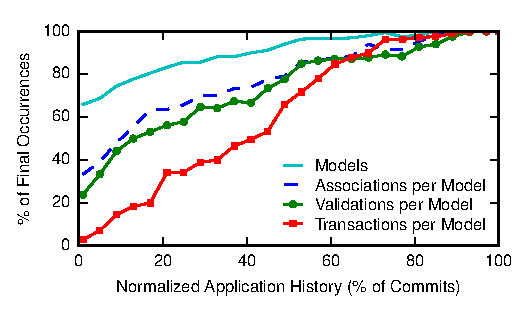
\includegraphics[width=\figscale\columnwidth]{figs/historical-median.pdf} \caption{Use of mechanisms over each project's history. We plot the median value of each metric across projects and, for each mechanism, omit projects that do not contain any uses of the mechanism (e.g., if a project lacks transactions, the project is omitted from the median calculation for transactions).}  \label{fig:historical} \end{figure}

\begin{figure}[h!]
  \newcommand{\skipht}{\\[-2em]}
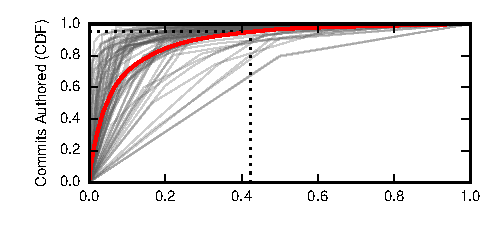
\includegraphics[width=\figscale\columnwidth]{figs/commit-authorship-cdf.pdf}\vspace{-1.5em}
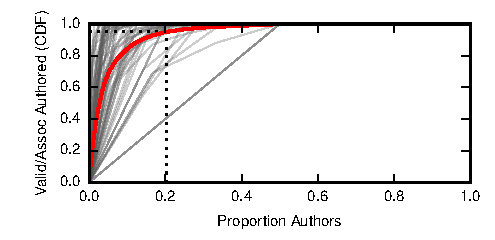
\includegraphics[width=\figscale\columnwidth]{figs/invariant-authorship-cdf.pdf}
\caption{CDFs of authorship of invariants (validations plus
  associations) and commits. Bolded line
  shows the average CDF across projects, while faint lines show CDFs
  for individual projects. The dotted line shows the 95th percentile
  CDF value. }
\label{fig:cdfs}
\end{figure}


Overwhelmingly, applications did not use transactions or locks
(Figure~\ref{fig:usages} and Table~\ref{table:app-summary}). On
average, applications used 0.13 transactions, 0.01 locks, 1.80
validations, and 3.19 associations per model (with an average of 29.1
models per application). While 46 (68.7\%) of applications used
transactions, all used some validations or associations. Only six
applications used locks. Use of pessimistic locks was over twice
as common as the use of optimistic locks.

Perhaps most notable among these general trends, we find that
validations and associations are, respectively, 13.6 and 24.2 times
more common than transactions and orders of magnitude more common than
locking. These feral mechanisms are---in keeping with the Rails
philosophy---favored by these application developers. That is, rather
than adopting the use of traditional transactional programming
primitives, Rails application writers chose to instead specify
correctness criteria and have the ORM system enforce the criteria on
their behalf. It is unclear and even unlikely that these declarative
criteria are a complete specification of program correctness:
undoubtedly, some of these programs contain errors and omissions. However, given
that these criteria are nevertheless being declared by application
writers and represent a departure from traditional,
transaction-oriented programming, we devote much of the remainder of
this work to examining exactly what they are attempting to preserve
(and whether they are actually sufficient to do so).

\minihead{Understanding specific applications} Over the course of our
investigation, we found that application use of mechanisms
varied. While our focus is largely on aggregate behavior, studying
individual applications is also interesting. For example, consider
Spree, a popular eCommerce application:

Spree uses only six transactions, one for each of $1.)$ canceling an
order, $2.)$ approving an order (atomically setting the user ID and
timestamp), $3.)$ transferring shipments between fulfillment locations
(e.g., warehouses), $4.)$ transferring items between shipments, $5.)$
transferring stock between fulfillment locations, and $6.)$ updating an
order's specific inventory status. While this is a reasonable set of
locations for transactions, in an eCommerce application, one might
expect a larger number of scenarios to require transactions, including
order placement and stock adjustment.

In the case of Spree stock adjustment, the inventory count for each
item is a potential hotspot for concurrency issues. Manual adjustments
of stock that is available (``adjust\_count\_on\_hand'') is indeed
protected via a pessimistic lock, but simply setting the amount of
stock that is available (``set\_count\_on\_hand'') is not. It is
unclear why one operation necessitates a lock but the other does not,
given that both are ostensibly sensitive to concurrent
accesses. Meanwhile, the stock level field is wrapped in a validation
ensuring non-negative balances, preventing negative balances but not
necessarily classic Lost Update anomalies~\cite{adya}.

At one point, Spree's inventory count was protected by an optimistic
lock; it was removed due to optimistic lock failure during customer
checkouts. On relevant GitHub issue pertaining to this lock removal, a
committer notes that ``I think we should get rid of the [optimistic
lock] if there's no documentation about why it's there...I think we
can look at this issue again in a month's time and see if there's been
any problems since you turned it
off''~\cite{code-optimistic-issue}. This removal has, to our
knowledge, not been revisited, despite the potential dangers of
removing this point of synchronization.

The remainder of the application corpus contains a number of such
fascinating examples, illustrating the often ad-hoc process of
deciding upon a concurrency control mechanism. Broadly, the use of
each style of concurrency control varies across repositories, but our
results demonstrate a clear trend towards feral mechanisms within
Rails rather than traditional use of transactions.

\begin{figure}
  \newcommand{\skipht}{\\[-1em]}
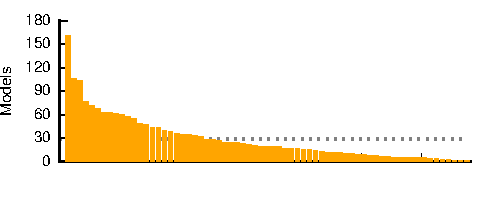
\includegraphics[width=.75\columnwidth]{figs/models-single-bar.pdf}\skipht
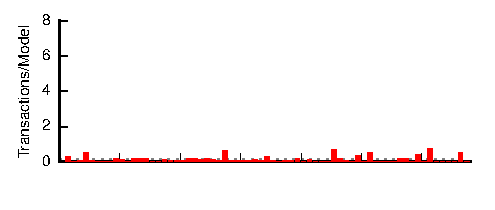
\includegraphics[width=.75\columnwidth]{figs/transactions-single-bar.pdf}\skipht
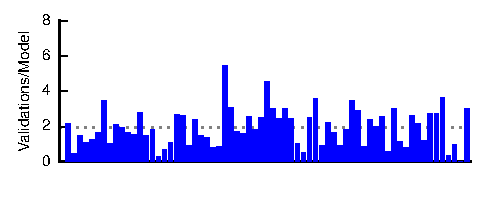
\includegraphics[width=.75\columnwidth]{figs/validations-single-bar.pdf}\skipht
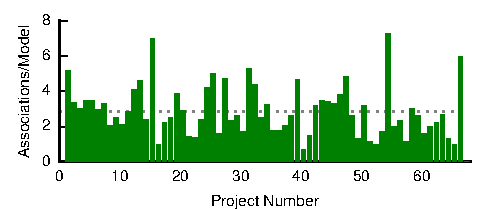
\includegraphics[width=.75\columnwidth]{figs/associations-single-bar.pdf}\\\vspace{.5em}
\caption{Use of concurrency control mechanisms in Rails
  applications. We maintain the same ordering of applications for each
  plot (i.e., same x-axis values; identical to
  Table~\ref{table:app-summary}) and show the average for each plot
  using the dotted line.}
\label{fig:usages}
\end{figure}



\minihead{Additional metrics} To better understand how programmers
used each of these mechanisms, we performed two additional
analyses.

First, we analyzed the number of models, transactions, validations,
and associations over each project's lifetime. Using each project's
Git history, we repeated the above analysis at a fixed set of
intervals through the project's lifespan (measured by
commits). Figure~\ref{fig:historical} plots the median
number of occurrences across all projects. The results show that
concurrency control mechanisms (of all forms) tend to be introduced
after models are introduced. That is, additions to the data model
precede (often by a considerable amount) additional uses of
transactions, validations, and associations. It is unclear whether the
bulk of concurrency control usage additions are intended to correct
concurrency issues or are instead due to natural growth in Controller
code and business logic. However, the gap between models and
concurrency control usage shrinks over time; thus, the data model
appears to stabilize faster than the controller logic, but both
eventually stabilize. We view additional longitudinal analysis along
these lines as worthwhile future work.


Second, we analyze the distribution of authors to commits compared to
the distribution of authors to validations and associations
authored.\footnote{We chose to analyze commits authored rather than
  lines of code written because git tracks large-scale code
  refactoring commits as an often large set of deletions and
  insertions. Nevertheless, we observed a close correlation between
  lines of code and commits authored.} As Figure~\ref{fig:cdfs} (see
Appendix, page~\pageref{fig:cdfs}) demonstrates, 95\% of all commits
are authored by 42.4\% of authors. However, 95\% of invariants
(validations plus associations) are authored by only 20.3\% of
authors. This is reminiscent of database schema authorship, where,
traditionally, a smaller number of authors (e.g., DBAs) modify the
schema than contribute to the actual application code.


\FloatBarrier
\subsubsection{Summary and Discussion}

Returning to the Rails design philosophy, the applications we have
encountered do indeed express their logic at the application
layer. There is little actual communication of correctness criteria to
the database layer. Part of this is due to limitations within
Rails. As we have mentioned, there is no way to actually declare a
foreign key constraint in Rails without importing additional
third-party modules. Insofar as Rails is an ``opinionated'' framework
encouraging an idiomatic programming style, if our application corpus
is any indication, DHH and his co-authors advocating application-level
data management appear to have succeeded en masse.

Having observed the relative popularity of these mechanisms, we turn
our attention to the question of their correctness. Specifically, do
these application-level criteria actually enforce the constraints that
they claim to enforce? We restrict ourself to studying declared
validations and associations for three reasons. First, as we have
seen, these constructs are more widely used in the codebases we have
studied. Second, these constructs represent a deviation from standard
concurrency control techniques and are therefore perhaps more likely
to contain errors. Third, while analyzing latent constraints (e.g.,
those that might be determined via more sophisticated techniques such
as pre- and post-condition invariant
mining~\cite{homeostasis,redblue-new} and/or by interviewing each
developer on each project) would be instructive, this is difficult to
scale. We view these forms of analysis as highly promising avenues for
future research.


\subsection{Rails \IConfluence Analysis}
\label{sec:apps}

We now turn our attention to understanding which of Rails' feral
validations and associations are actually correct under concurrent
execution as described in Section~\ref{sec:deployment} and which
require stronger forms of isolation or synchronization for correct
enforcement.

\subsubsection{Understanding Validation Behavior}

To begin, recall that each sequence of validations (and model update
as well, if validations pass) is wrapped within a database-backed
transaction, the validation's intended integrity will be preserved
provided the database is using serializable isolation. However,
relational database engines often default to non-serializable
isolation~\cite{hat-vldb}; notably for Rails, PostgreSQL and MySQL
actually default to, respectively, the weaker Read Committed and
Repeatable Read isolation levels.

We did not encounter evidence that applications changed the isolation
level. Rails does not configure the database isolation level for
validations, and none of the application code or configurations we
encountered change the default isolation level, either (or mention
doing so in documentation). Thus, although we cannot prove that this
is indeed the case, this data suggests that validations are likely
to run at default database isolation in production environments.

\minihead{Validations with weak isolation} Given that validations are
not likely to be perfectly isolated, does this lack of serializable
isolation actually affect these invariants?  Just because validations
effectively run concurrently does not mean that they are necessarily
incorrect. To determine exactly which of these invariants are correct
under concurrent execution, we employ \iconfluence analysis. In the
case of Rails, we wish to determine whether, in the event of
concurrent validations and model saves, the result of concurrent model
saves will not violate the validation for either model. In the event
that two concurrent controllers save objects that are backed by the
same database record, only one will be persisted (a some-write-wins
``merge''). In the event that two concurrent controllers save
different models (i.e., backed by different database records), both
will be persisted (a set-based ``merge''). In both cases, we must
ensure that validations hold after merge.

Per above, our \iconfluence analysis currently relies on a combination
of manual proofs and simple static analysis: given a set of invariant
and operation pairs classified as providing the \iconfluence property,
we can iterate through all operations and declared invariants and
check whether or not they appear in the set of \iconfluent pairs. If
so, we label the pair as \iconfluent. If not, we can either
conservatively label the pair as unsafe under concurrent execution or
prove the pair as \iconfluent or not. (To prove a pair is \iconfluent,
we must show that the set of database states reachable by executing
operations preserves the invariant under merge, as described above.)

Returning to our task of classifying Rails validations and
associations as safe or not, we applied this \iconfluence analysis to
the invariants\footnote{We focus on validations here as, while
  associations \textit{do} represent an invariant, it is only when
  they are coupled with validations that they are enforced.} in the
corpus. In our analysis, we
found that only 60 out of 3505 validations were expressed as
user-defined functions. The remainder were drawn from the standard set
of validations supported by Rails core.\footnote{It is unclear exactly
  why this is the case. It is possible that, because these invariants
  are standardized, they are more accessible to users. It is also
  possible that Rails developers have simply done a good job of
  codifying common patterns that programmers tend to use.}
Accordingly, we begin by considering built-in validations, then
examine each of the custom validations.

\subsubsection{Built-In Validations}

We now discuss common, built-in validations and their
\iconfluence. Many are \iconfluent and are therefore safe to execute
concurrently.

Table~\ref{table:builtins} presents the ten most common built-in
validations by usage and their occurrences in our application
corpus. The exact coordination requirements depended on their usage.

The most popular invariant, \texttt{presence}, serves multiple purposes. Its
basic behavior is to simply check for empty values in a model before
saving. This is \iconfluent as, in our model, concurrent model saves
cannot result in non-null values suddenly becoming null. However,
\texttt{presence} can also be used to enforce that the opposite end of
an association is, in fact, present in the database (i.e., referential
integrity). Under insertions, foreign key constraints are
\iconfluent~\cite{coord-avoid}, but, under deletions, they are not.

The second most popular invariant, concerning record uniqueness, is
\textit{not} \iconfluent~\cite{coord-avoid}. That is, if two users
concurrently insert or modify records, they can introduce duplicates.

Eight of the next nine invariants are largely concerned with data
formatting and are \iconfluent. For example, \texttt{numericality}
ensures that the field contains a number rather than an alphanumeric
string. These invariants are indeed \iconfluent under concurrent
update.

Finally, the safety of \texttt{associated} (like \texttt{presence}) is
contingent on whether or not the current updates are both insertions
(\iconfluent) or mixed insertions and deletions (not
\iconfluent). Thus, correctness depends on the operation.

Overall, a large number of built-in validations are safe under
concurrent operation. Under insertions, 86.9\% of built-in validation
occurrences as \iconfluent. Under deletions, only 36.6\% of
occurrences are \iconfluent.  However, associations and multi-record
uniqueness are---depending on the workload---not \iconfluent and are
therefore likely to cause problems. In the next section, we examine
these validations in greater detail.

\begin{table}
\begin{center}
\small
\begin{tabular}{|l l l |}
\hline
Name & Occurrences & I-Confluent?\\\hline
\texttt{validates\_presence\_of} & 1762 & Depends\\
\texttt{validates\_uniqueness\_of} & 440 & No \\
\texttt{validates\_length\_of} & 438 & Yes \\
\texttt{validates\_inclusion\_of} & 201 & Yes\\
\texttt{validates\_numericality\_of} & 133 & Yes \\
\texttt{validates\_associated} & 39 & Depends\\
\texttt{validates\_email} & 34 & Yes \\
\texttt{validates\_attachment\_content\_type} & 29 & Yes \\
\texttt{validates\_attachment\_size} & 29 & Yes \\
\texttt{validates\_confirmation\_of} & 19 & Yes \\
Other & 321 & Mixed \\\hline
\end{tabular}
\end{center}\vspace{-.5em}
\caption{Use of and \iconfluence of built-in validations.}
\label{table:builtins}
\end{table}

\subsubsection{Custom Validations}

We also manually inspected the coordination requirements of the 60
(1.71\%) validations (from 17 projects) that were declared as UDFs. 52
of these custom validations were declared inline via Rails's
\texttt{validates\_each} syntax, while 8 were custom classes that
implemented Rails's validation interface. 42 of 60 validations were
\iconfluent, while the remaining 18 were not. Due to space
constraints, we omit a discussion of each validation but discuss
several trends and notable examples of custom validations below.

Among the custom validations that were \iconfluent, many consisted of
simple format checks or other domain-specific validations, including
credit card formatting and static username blacklisting.

The validations that were not \iconfluent took on a range of
forms. Three validations performed the equivalent of foreign key
checking, which, as we have discussed, is unsafe under deletion. Three
validations checked database-backed configuration options including
the maximum allowed file upload size and default tax rate; while
configuration updates are ostensibly rare, the outcome of each
validation could be affected under a configuration change. Two
validations were especially interesting. Spree's
\texttt{AvailabilityValidator} checks whether an eCommerce inventory
has sufficient stock available to fulfill an order; concurrent order
placement might result in negative stock. Discourse's
\texttt{PostValidator} checks whether a user has been spamming the
forum; while not necessarily critical, a spammer could technically
foil this validation by attempting to simultaneously author many posts.

In summary, again, a large proportion of validations appear
safe. Nevertheless, the few non-\iconfluent validations should be
cause for concern under concurrent execution.



\section{Quantifying Integrity Violations in Rails}
\label{sec:feral-evaluation}

While many of the validations we encountered were \iconfluent,
not all were. In this section, we specifically investigate the effect
of concurrent execution on two of the most popular non-\iconfluent
validations: uniqueness and foreign key validations.

\subsubsection{Uniqueness Constraints and Isolation}

To begin, we consider Rails's uniqueness validations: 12.7\% of the
built-in validation uses we encountered. In this section, we discuss
how Rails implements uniqueness and show that this is---at least
theoretically---unsafe.

When a model field is declared with a \texttt{:validates\_uniqueness}
annotation, any instance of that model is compared against all other
corresponding records in the database to ensure that the field is
indeed unique. ActiveRecord accomplishes this by issuing a
``\texttt{SELECT}'' query in SQL and, if no such record is found,
Rails updates the instance state in the database
(Appendix~\ref{sec:appendix-uniqueness-behavior}).

While this user-level uniqueness validation runs within a transaction,
the isolation level of the transaction affects its
correctness. For correct execution, the \texttt{SELECT} query must
effectively attain a predicate lock on the validated column for the
duration of the transaction. This behavior \textit{is} supported under
serializable isolation. However, under Read Committed or Repeatable
Read isolation, no such mutual exclusion will be performed, leading to
potential inconsistency.\footnote{Using \texttt{SELECT FOR UPDATE}
  under these weaker models would be safe, but Rails does not
  implement its predicate-based lookups as such (i.e., it instead opts
  for a simple \texttt{SELECT} statement).}  Moreover, validation under Snapshot Isolation
may similarly result in
inconsistencies.\footnote{The first reference to the potential integrity
  violations resulting from this implementation in the Rails code that
  we are aware of dates to December 2007, in Rails
  v.2.0.0~\cite{code-unique-race-one}.  In September 2008, another
  user added additional discussion within the code comments, noting
  that ``this could even happen if you use transactions with the
  'serializable' isolation
  level''~\cite{code-unique-race-two}. The use of ``'serializable''' suggests familiarity with the
  common, erroneous labeling of Snapshot Isolation as ``serializable''
  (as in Oracle 12c documentation and PostgreSQL documentation prior
  to the introduction of SSI in version 9.1.1 in September
  2011)\label{fn:si-rails}. } Thus, unless the database is configured
for serializable isolation, integrity violations may result.

As we have discussed, MySQL and PostgreSQL each support serializable
isolation but default to weaker isolation. Moreover, in our
investigation, we discovered a bug in PostgreSQL's implementation of
Serializable Snapshot Isolation that allowed duplicate records to be
created under serializable isolation when running a set of
transactions derived from the Rails primary key validator. We have
confirmed this anomalous behavior with the core PostgreSQL
developers\footnote{``BUG \#11732: Non-serializable outcomes under
  serializable isolation'' at
  \url{http://www.postgresql.org/message-id/20141021071458.2678.9080@wrigleys.postgresql.org}\label{fn:pg-bug}}
and, as of March 2015, the behavior persists. Thus, any discussion of
weak isolation levels aside, PostgreSQL's implementation of
serializability is non-serializable and is insufficient to provide
correct behavior for Rails' uniqueness validations. So-called
``serializable'' databases such as Oracle 12c that actually provide
Snapshot Isolation will similarly fall prey to duplicate validations.

The Rails documentation warns that uniqueness validations may fail and
admit duplicate records~\cite{rails-guide}. Yet, despite the
availability of patches that remedy this behavior by the use of an
in-database constraint and/or index, Rails provides this incorrect
behavior by default. (One patch was rejected; a developer reports
``[t]he reasons for it not being incorporated...are lost in the mists
of time but I suspect it's to do with backwards compatibility, cross
database compatibility and applications varying on how they want/need
to handle these kind of errors.''~\cite{code-index-patch}).

In another bug report complaining of duplicates due to concurrent
uniqueness validation, a commenter asserts ``this is not a bug but
documented and inherent behavior of
validates\_uniqueness\_of''~\cite{code-index-error}.  A Rails
committer follows up, noting that ``the only way to handle
[uniqueness] properly is at the database layer with a unique
constraint on the column,'' and subsequently closes the issue. The
original bug reporter protests that ``the problem extends beyond
unique constraints and into validations that are unique to a Rails
application that can't [sic?!]  be enforced on the DB level''; the
Rails committer responds that ``with the possible exception of
[associations,] all of the other validations are constrained by the
attribute values currently in memory, so aren't susceptible to similar
flaws.'' This final statement is correct for many of the built-in
validations but is not correct for arbitrary user-defined
validations. We discuss the user-defined validation issue further in
Section~\ref{sec:rails-discussion}.

\minihead{Understanding validation behavior} Given that entirely feral
mechanisms can introduce duplicates, how many duplicates can be
introduced? Once a record is written, any later validations will
observe it via \texttt{SELECT} calls. However, \textit{while} a record
is being validated, any number of concurrent validations can
unsafely proceed. In practice, the number of concurrent validations
is dependent on the Rails environment. In a Rails deployment
permitting $P$ concurrent validations (e.g., a single-threaded,
multi-process environment with $P$ processes), each value in the
domain of the model field/database column can be inserted no more than
$P$ times. Thus, validations---at least theoretically---bound the
worst-case number of duplicate records for each unique value in the
database table.

\subsubsection{Quantifying Uniqueness Anomalies}

Given that feral uniqueness validations are acknowledged to be unsafe
under non-serializable isolation yet are widely used, we sought to
understand exactly how often uniqueness anomalies occur in an
experimental deployment. In this section, we demonstrate that
uniqueness validations in Rails are indeed unsafe under
non-serializable isolation. While they prevent some data integrity
errors, we observe---depending on the workload---many duplicate
records.

\minihead{Experimental setup} We developed a Rails 4.1.5 application
that performed insertions to a non-indexed string column and compared
the incidence of violations both with and without a uniqueness
validator (see also
Appendix~\ref{sec:appendix-uniqueness-schema}).\footnote{In our
  experimental evaluation, we use the custom applications described
  in Section~\ref{sec:feral-details} for two
  reasons. First, these test cases allow us to isolate ActiveRecord
  behavior to the relevant set of validations as they are deployed by
  default, independent of any specialized controller logic. Second,
  this reduces the complexity of automated testing. Many of the
  applications in our corpus indeed use the same code paths within
  ActiveRecord, but evaluating these custom applications simplifies
  programmatic triggering of validation logic.} We deployed this
application on two Amazon EC2 \texttt{m2.4xlarge} instances, offering
68.4 GB RAM, 8 CPU cores, and 1680GB local storage, running Ubuntu
14.04 LTS. On one instance, we deployed our application, using Nginx
1.6.2 as a web frontend proxied to a set of Unicorn 4.8.3 (Ruby VM
pool) workers. Nginx acts as a HTTP frontend and forwards incoming
requests to a variably sized pool of Rails VMs (managed by Unicorn, in
a multi-process, single-threaded server) that \texttt{epoll} on a
shared Linux file descriptor. On the other EC2 instance, we deployed
PostgreSQL 9.3.5 and configured it to run on the instance local
storage. We used a third EC2 instance to direct traffic to the
front-end instance and drive load. We plot the average and standard
deviation of three runs per experiment.

\minihead{Stress test} We began our study by issuing a simple stress
test that executed a number of concurrent insertion requests against a
variable number of Unicorn workers. We repeatedly issued a set of 64
concurrent model creation (SQL insertion) requests, each with the same
validated key (e.g., all with field \texttt{key} set to value 1)
against the Rails application. Across an increasing number of Unicorn
workers, we repeated this set of requests 100 times (blocking
in-between rounds to ensure that each round is, in fact, a concurrent
set of requests), changing the validated key each round
(Appendix~\ref{sec:appendix-uniqueness-stress}).

Figure~\ref{fig:pk-stress} shows the results. With no validation, all
concurrent requests succeed, resulting in 6300 duplicate records (100
rounds of 64-1 duplicate keys). With validations enabled, the number
of violations depends on the degree of concurrency allowed by
Unicorn. With only one process, Unicorn performs the validations
serially, creating no duplicates. However, with two processes, Unicorn
processes race, resulting in 70 duplicate records spread across 70
keys. With three processes, Unicorn produces 249 duplicate records
across all 100 keys. The number of duplicates increases with the
number of processes, peaking at 16 workers. With additional workers,
duplicate counts decrease slightly, which we attribute to thrashing
between workers and within PostgreSQL (recall that each instance has
only 8 cores). Nevertheless, using validations, the microbenchmark
duplicate count remains below 700---nearly an order-of-magnitude fewer
duplicates than without using validations. Therefore, even though
these validations are incorrectly implemented, they still
result in fewer anomalies. However, when we added in in-database
unique index on the \texttt{key} column\footnote{In this case, we
  added a unique index to the model using Active Record's
  \textit{database migration}, or manual schema change
  functionality. Migrations are written separately from the Active
  Record model declarations. Adding the index was not difficult, but,
  nevertheless, the index addition logic is separate from the domain
  model. Without using third-party models, we are unaware of a way to
  enforce uniqueness within Rails without first declaring an index
  that is \textit{also} annotated with a special \texttt{unique: true}
  attribute.} and repeated the experiment, we observed no duplicates,
as expected.

\begin{figure}
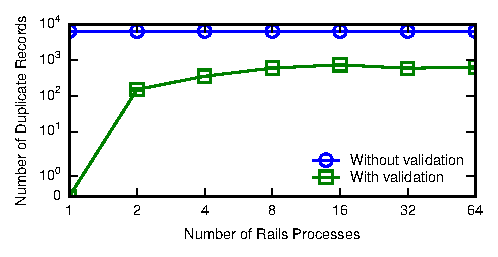
\includegraphics[width=\figscale\columnwidth]{figs/pk_stress_violations.pdf}
\caption{Uniqueness stress test integrity violations.}
\label{fig:pk-stress}
\end{figure} 

\minihead{Actual workloads} The preceding experiment stressed a
particularly high-contention workload---in effect, a worst case
workload for uniqueness validations. In practice, such a workload is
likely rare.\footnote{In fact, it was in the above workload that we
  encountered the non-serializable PostgreSQL behavior under
  serializable isolation. Under serializable isolation, the number of
  anomalies is reduced compared to the number under Read Committed
  isolation (as we report here), but we still detected duplicate
  records.} Accordingly, we set up another workload meant to capture a
less pathological access pattern. We ran another insert-only workload,
with key choice distributed among a fixed set of keys. By varying the
distribution and number of keys, we were able to both capture more
realistic workloads and also control the amount of contention in the
workload. As a basis for comparison, we ran four different
distributions. First, we considered uniform key access. Second, we
used YCSB's Zipfian-distributed accesses from
\texttt{workloada}~\cite{ycsb}. Third and fourth, we used the item
distribution access from Facebook's LinkBench workload, which captures
MySQL record access when serving Facebook's social
graph~\cite{linkbench}. Specifically, we used---separately---the
insert and update traffic from this benchmark.

For each trial in this workload, we used 64 concurrent clients
independently issuing a set of 100 requests each, with a fixed number
of 64 Unicorn workers per process (Appendix~\ref{sec:appendix-uniqueness-workload}). 

Figure~\ref{fig:pk-workload} illustrates the number of duplicate
records observed under each of these workloads. As we increase the
number of possible keys, there are two opposing effects. With more
keys, the probability of any two operations colliding
decreases. However, recall that, once a key is written, all subsequent
validators can read it. While
the uniform workload observes an average of 2.33 duplicate records
with only one possible key, it observes an average of 26 duplicate
keys with 1000 possible keys. Nevertheless, with 1 million possible
keys, we do not observe any duplicate records.

The actual ``production'' workloads exhibit different trends. In
general, YCSB is an extremely high contention workload, with a Zipfian
constant of 0.99, resulting in one very hot key. This decreases the
beneficial effect of increasing the number of keys in the
database. However, LinkBench has less contention and anomalies decrease more
rapidly with increased numbers of keys.

\begin{figure}
\begin{center}
\hspace{4em}
\begin{minipage}[l]{0cm}

\includegraphics[angle=90, width=.23in]{figs/pk-workload-ylabel.pdf}
\end{minipage}
\begin{minipage}{\figscale\columnwidth}
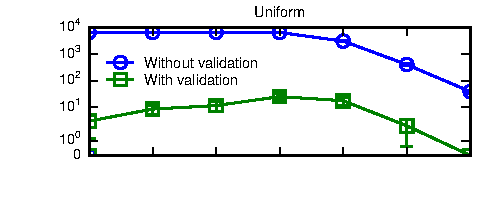
\includegraphics[width=\figscale\columnwidth]{figs/pk-workload-uniform-violations.pdf}\vspace{-1em}
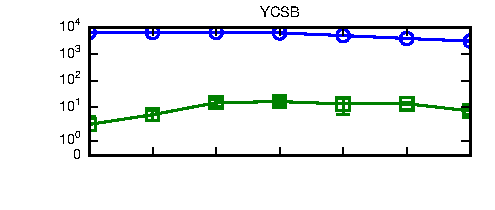
\includegraphics[width=\figscale\columnwidth]{figs/pk-workload-ycsb-violations.pdf}\vspace{-1em}
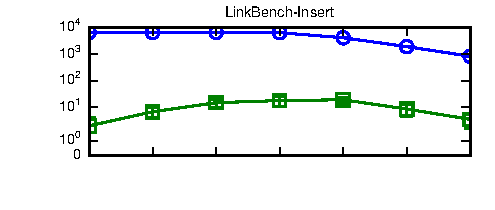
\includegraphics[width=\figscale\columnwidth]{figs/pk-workload-linkbench-ins-violations.pdf}\vspace{-1em}
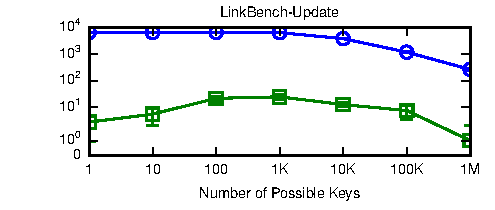
\includegraphics[width=\figscale\columnwidth]{figs/pk-workload-linkbench-upd-violations.pdf}
\end{minipage}\vspace{.5em}
\caption{Uniqueness workload integrity violations.}
\label{fig:pk-workload}
\end{center}
\end{figure}

\subsubsection{Association Validations and Isolation}

Having investigated uniqueness constraints, we turn our attention to
association validations. We first, again, discuss how Rails enforces
these validations and describe how---at least
theoretically---validations might result in integrity errors.

When a model field is declared with an association (e.g., it
\texttt{:belongs\_to} another model) \textit{and} a
\texttt{:validates\_presence} validation, Rails will attempt to ensure
that the declared validation is valid before saving the model. Rails
accomplishes this by issuing a ``\texttt{SELECT WHERE}'' query in SQL
to find an associated record (e.g., to ensure the ``one'' end of a
one-to-many relationship exists) and, if a matching association is
found, Rails updates the instance state in the database
(Appendix~\ref{sec:appendix-association-behavior}). On deletion, any
models with associations marked with \texttt{:dependent => destroy}
(or \texttt{:dependent => delete}) will have any associated models
destroyed (i.e., removed by instantiating in Rails and calling
\texttt{destroy} on the model) or deleted (i.e., removed by simply
calling the database's \texttt{DELETE} method).

This feral association validation runs within a transaction, but,
again the exact isolation level of the transaction affects its
correctness. For correct execution, the \texttt{SELECT} query must
also attain a predicate lock on the specific value of the validated
column for the duration of the transaction. Similar to the uniqueness
validator, concurrent deletions and insertions are unsafe under Read
Committed, Repeatable Read, and Snapshot Isolation. Thus, unless the
database is configured for serializable isolation, inconsistency may
result and the feral validation will fail to prevent data corruption.

Unlike uniqueness validations, there is no discussion of associations
and concurrency anomalies in the Rails documentation. Moreover, in
Rails 4.1, there is no way to natively declare a foreign key
constraint;\footnote{Rails 4.2 added support for foreign keys via
  migration annotation (separate from models; similarly to adding a
  unique index) in December 2014.} it must be done via a third-party
library such as \texttt{foreigner}~\cite{foreigner} or
\texttt{schema\_plus}~\cite{schemaplus}. Only two applications
(\texttt{canvaslms} and \texttt{diaspora}) used \texttt{foreigner},
and only one application (\texttt{juvia}) used
\texttt{schema\_plus}. One application (\texttt{jobsworth}) used a
custom schema annotation and constraint generator.

\minihead{Understanding association behavior} Given that entirely
feral mechanisms can introduce broken associations, how many dangling
records can be introduced? Once a record is deleted, any later
validations will observe it via \texttt{SELECT} calls. However, in the
worst case, the feral cascading deletion on the one side of a
one-to-many relation can stall indefinitely, allowing an unlimited
number of concurrent insertions to the many side of the
relation. Thus, validations---at least theoretically---only reduce the
worst-case number of dangling records that were inserted prior to
deletion; any number of concurrent insertions may occur during
validation, leading to unbounded numbers of dangling records.

\subsubsection{Quantifying Association Anomalies}

Given this potential for errors, we again set out to quantify
integrity errors. We demonstrate that weak isolation can indeed lead
to data integrity errors in Rails' implementation of associations.

We performed another set of experiments to test association validation
behavior under concurrent insertions and deletions. Using the same
Unicorn and PostgreSQL deployment as above, we configured another
application to test whether or not Rails validations would correctly
enforce association-based integrity constraints. We consider an
application with two models: Users and Departments. We configure a
one-to-many relationship: each user \texttt{belongs\_to} a department,
and each department \texttt{has\_many} user
(Appendix~\ref{sec:appendix-association-schema}).

As a basic stress test, we initialize the database by creating 100
departments with no users. Subsequently, for each department in the
database, we issue a single request to delete the department along
with 64 concurrent requests to insert users in that department. To
correctly preserve the one-to-many relationship, the database should
either reject the deletion operation or perform a cascading deletion
of the department and any users (while rejecting any future user
creation requests for that department). We can quantify the degree of
inconsistency by counting the number of users left in the database who
have no corresponding department (Appendix~\ref{sec:appendix-association-stress}).

With associations declared in Rails, the Rails process performing the
deletion will attempt a cascading delete of users upon department
deletion. However, this cascade is performed, again, ferally---at the
application level. Thus, under non-serializable isolation, any user creation
events that are processed while the search for Users to delete is
underway will result in Users without departments.

Figure~\ref{fig:fk-stress} shows the number of ``orphaned'' Users
(i.e., Users without a matching Department) as a function of Rails
worker processes. With no constraints declared to Rails or to the
database, all User creations succeed, resulting in 6400 dangling
Users. With constraints declared in Rails (via a mix of validation and
association), the degree of inconsistency depends on the degree of
parallelism. Under the worst case, with 64 concurrent processes, the
validations are almost worthless in preventing integrity errors. In
contrast, when we declare a foreign key constraint within the
database\footnote{In this case, we introduced the constraint via SQL
  using a direct connection to the database. This change was
  straightforward but---like the unique index addition---was not
  reflected in the base Active Record models.}  and run the workload
again, we observe no inconsistency.

\begin{figure}
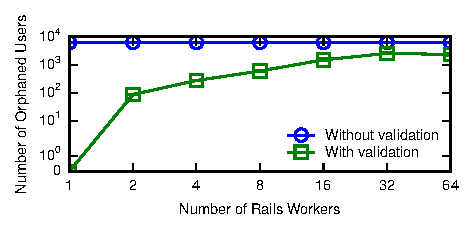
\includegraphics[width=\figscale\columnwidth]{figs/fk-stress-violations.pdf}
\caption{Foreign key stress association anomalies.}
\label{fig:fk-stress}
\end{figure}

The above stress test shows that inconsistency due to feral
concurrency control occurs only during times of contention---parallel
deletions and insertions. We subsequently varied the degree of
contention within the workload. We configured the same application and
performed a set of insertions and deletions, but spread across a
greater number of keys and at random. A set of 64 processes
concurrently each issued 100 User creation and Department deletion
requests (at a ratio of 10 to 1) to a set of randomly-selected keys
(again at a ratio of 10 Users to each Department). By varying the
number of Users and Departments, we were able to control the amount of
contention within the workload. Under this workload, inconsistency
resulted only when a Department deletion proceeded concurrently with a
User creation event and the feral cascading deletion ``missed'' the
User creation (Appendix~\ref{sec:appendix-association-workload}).

Figure~\ref{fig:fk-workload} shows the results. As the number of
Departments increases, we observe two trends. First, with only one
Department, there is again less chance of inconsistency: all
operations contend on the same data item, so the total number of
inconsistent, orphaned users is limited by the number of potentially
racing. However, as the number of Departments increases, the chance of
concurrent deletions and insertions drops.

\begin{figure}
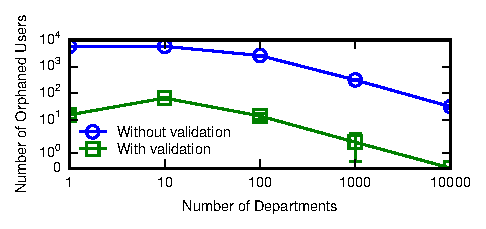
\includegraphics[width=\figscale\columnwidth]{figs/fk-workload-violations.pdf}
\caption{Foreign key workload association anomalies.}
\label{fig:fk-workload}
\end{figure}

\subsubsection{Takeaways and Discussion}

The preceding experiments demonstrate that, indeed, Active Record is
unsafe as deployed by default. Validations are susceptible to data
corruption due to sensitivity to weak isolation anomalies.

This raises the question: why declare validations at all? As we
observe, validations protect against \textit{some} data
corruption. First, they correctly guard against
non-concurrency-related anomalies such as data entry or input
errors. For example, if a user attempts to reserve a username that was
previously chosen, a validation would succeed. This basic
functionality is reasonably left to the ORM engine for
implementation. The failures we observe here are solely due to
concurrent execution. Without concurrent execution, validations are
correct. Second, validations \textit{do} reduce the incidence of
inconsistency. Empirically, even under worst-case workloads, these
validations result in order-of-magnitude reductions in
inconsistency. Under less pathological workloads, they may eliminate
it with high probability. It is possible that, in fact, the degree of
concurrency and data contention within Rails-backed applications
simply does not lead to these concurrency races---that, in some sense,
validations are ``good enough'' for many applications.

Nevertheless, in both cases, Rails's feral mechanisms are a poor
substitute for their respective database counterparts---at least in
terms of integrity. We re-examine the Rails community's reluctance to
embrace these mechanisms in Section~\ref{sec:rails-discussion}.




\section{Other Frameworks}
\label{sec:other-orms}

While our primary focus in this paper is Rails, we investigated
support for uniqueness, foreign key, and custom validations in several
other ORM frameworks. We find widespread support for validations and
varying susceptibility to integrity errors.

\newcommand{\orm}[1]{{\vspace{.45em}\noindent\textit{#1}}}

\orm{Java Persistence API} (JPA; version EE 7)~\cite{code-jpa} is a
standard Java Object persistence interface and supports both
uniqueness and primary key constraints in the database via specialized
object annotations. Thus, when JPA is used to create a table, it will
use the database to enforce these constraints. In 2009, JPA introduced
support for UDF validations via a JavaBean
interface~\cite{code-bean-validation}. Interestingly, both the
original (and current) Bean validation specifications specifically
address the use of uniqueness validations in their notes:\vspace{-.25em}
\begin{quote}
``Question: should we add @Unique that would map to @Column(unique=true)?
@Unique cannot be tested at the Java level reliably but could generate
a database unique constraint generation. @Unique is not part
of the [Bean Validation] spec today.''~\cite{jsr-bean}\vspace{-.25em}
\end{quote}
An author of a portion of the code specification notes separately:\vspace{-.25em}
\begin{quote}
  ``The reason @Unique is not part of the built-in constraints is the
  fact that accessing the [database] during a valiation [sic] is
  opening yourself up for potenital [sic] phantom reads. Think twice
  before you go for [an application-level] approach.''~\cite{unique-bean}\vspace{-.25em}
\end{quote}
%http://download.oracle.com/otn-pub/jcp/persistence-2.0-fr-eval-oth-JSpec/persistence-2_0-final-spec.pdf?AuthParam=1414639627_4654729130380ec6809634192c3faacb
By default, JPA Validations are run upon model save and run in a
transaction at the default isolation level, and therefore, as the
developers above hint, are susceptible to the same kinds of integrity
violations we study here.

\orm{Hibernate} (version 4.3.7)~\cite{code-hibernate}, a Java ORM
based on JPA, does \textit{not} automatically enforce declared foreign
key relationships: if a foreign key constraint is declared; a
corresponding column is added, but that column is \textit{not} backed by a
database foreign key. Instead, for both uniqueness and foreign key
constraints, Hibernate relies on JPA schema annotations for
correctness. Therefore, without appropriate schema annotations,
Hibernate's basic associations may contain dangling references. Hibernate also has an extensive user-level validation
framework implementing the JPA Validation Bean
specification~\cite{code-hibernate-validator} and is sensitive to weak
isolation anomalies, similar to Rails validations.

\orm{CakePHP} (version 2.5.5)~\cite{code-cakephp}, a PHP-based web
framework, supports uniqueness, foreign key, and UDF
validations. CakePHP does \textit{not} back any of its validation
checking with a database transaction and relies on the user to
correctly specify any corresponding foreign keys or uniqueness
constraints within the database the schema. Thus, while users can
declare each of these validations, there is no guarantee that they are
actually enforced by the database. Thus, unless users are careful to
specify constraints in both their schema and in their validations,
validations may lead to integrity violations.

\orm{Laravel} (version 4.2)~\cite{code-laravel}, another PHP-based web
framework, supports the same set of functionality as CakePHP,
including application-level uniqueness, foreign key, and UDF
validations in the application. Any database-backed constraints must
be specified manually in the schema. Per one set of community
documentation~\cite{laravel-book}, ``database-level validations can
efficiently handle some things (such as uniqueness of a column in
heavily-used tables) that can be difficult to implement otherwise''
but ``testing and maintenance is more difficult...[and] your
validations would be database- and schema-specific, which makes
migrations or switching to another database backend more difficult in
the future.'' In contrast, model-level validations are ``the
recommended way to ensure that only valid data is saved into your
database. They are database agnostic, cannot be bypassed by end users,
and are convenient to test and maintain.'' 

\orm{Django} (version 1.7)~\cite{code-django}, a popular Python-based
framework, backs declared uniqueness and foreign key constraints with
database-level constraints. It also supports custom validations, but
these validations are not wrapped in a
transaction~\cite{code-django-constraints}. Thus, Django also appears
problematic, but only for custom validations.

\orm{Waterline} (version 0.10)~\cite{code-waterline}, the default ORM
for Sails.js (a popular MVC framework for Node.js~\cite{code-sails}),
provides support for in-DB foreign key and uniqueness constraints
(when supported by the database) as well as custom validations (that
are \textit{not} supported via transactions; e.g., ``TO-DO: This
should all be wrapped in a transaction. That's coming next but for the
meantime just hope we don't get in a nasty state where the operation
fails!''~\cite{code-waterline-txn}).

\minihead{Summary} In all, we observe common cross-framework support
for feral validation/invariants, with inconsistent use of mechanisms
for enforcing them, ranging from the use of in-database constraints to
transactions to no ostensible use of concurrency control in either
application or database.

% Implementing and using unique indexes~\cite{waterline-unique-one,waterline-unique-two}.

\begin{comment}

Name & PK & FK & UDF Validations
DJANGO & Automatic & Automatic & Yes
JPA & Yes, annotation & Yes, annotation & Yes, via Beans
CakePHP & 

% Django

Supports validations
https://docs.djangoproject.com/en/dev/ref/validators/

Broken online: http://stackoverflow.com/a/5690705


1.9 (not yet released) deprecating in favor of checks
https://docs.djangoproject.com/en/1.7/internals/deprecation/

checks:
https://docs.djangoproject.com/en/1.7/topics/checks/



%FK 

does it right
https://docs.djangoproject.com/en/1.7/ref/models/fields/#django.db.models.ForeignKey

%PK

does it right, by default declares an index
https://docs.djangoproject.com/en/1.7/_modules/django/db/backends/schema/


'''
If True, this field must be unique throughout the table.

This is enforced at the database level and by model validation. If you try to save a model with a duplicate value in a unique field, a django.db.IntegrityError will be raised by the model’s save() method.

This option is valid on all field types except ManyToManyField, OneToOneField, and FileField.

Note that when unique is True, you don’t need to specify db_index, because unique implies the creation of an index.
'''
a

% Hibernate/JPA


%FK 

no FK by default, relies on JPA
http://docs.jboss.org/hibernate/orm/4.3/manual/en-US/html/ch08.html

JoinColumn
http://docs.oracle.com/javaee/6/api/javax/persistence/OneToMany.html

%PK

``The reason @Unique is not part of the built-in constraints is the fact that accessing the Session/EntityManager during a valiation is opening yourself up for potenital phantom reads. Think twice before you go for the following approach.''
https://developer.jboss.org/wiki/AccessingtheHibernateSessionwithinaConstraintValidator?_sscc=t
http://stackoverflow.com/questions/17092601/validate-unique-username-in-spring

http://docs.oracle.com/javaee/6/api/javax/persistence/UniqueConstraint.html

BEAN supported
https://jcp.org/en/jsr/detail?id=303

%CakePHP
supports udf validations
http://book.cakephp.org/2.0/en/models/data-validation.html

basically you set up your own schema, but default validations don't
appear to be transactional

%FK 


%PK

https://github.com/cakephp/cakephp/blob/50b3893e6507979427e1aaeb435494aed1af4f52/lib/Cake/Model/Model.php#L3303


% Laravel

Manually define database schema!

%FK 
%PK

http://laravel.com/docs/4.2/validation#rule-unique
https://github.com/laravel/framework/blob/75b1dff27778354e44511556171cf6ae466c8b59/src/Illuminate/Validation/Validator.php#L940


http://laravelbook.com/laravel-input-validation/

% Node -- Sail.js
%FK 
%PK

Validations are handled by Anchor, a thin layer on top of Validator, one of the most robust validation libraries for Node.js. Sails supports most of the validations available in Validator, as well as a few extras that require database integration, like unique.

http://sailsjs.org/#/documentation/concepts/ORM/Validations.html
https://github.com/balderdashy/sails/issues/832

https://github.com/balderdashy/waterline

Broken in Mongo
https://github.com/balderdashy/sails-mongo/issues/152

Broken in dev
https://github.com/balderdashy/waterline/issues/55

Because you have migrate: safe set the indexes will not be created when you start the ORM.
https://github.com/balderdashy/waterline/issues/236

uses db foreign keys

\end{comment}

% what can we learn?
% udfs


\section{Implications for Databases}
\label{sec:feral-discussion}
\label{sec:rails-discussion}

In light of this empirical evidence of the continued mismatch between
ORM applications and databases, in this section, we reflect on the
core database limitations for application writers today and suggest a
set of directions for alleviating them.

\subsection{Summary: Database Shortcomings Today}

The use of feral invariants is not well-supported by today's
databases. At a high level, today's databases effectively offer two
primary options for ORM framework developers and users:

\begin{enumerate}
\item \textbf{Use ACID transactions.} Serializable transactions are
  sufficient to correctly enforce arbitrary application invariants,
  including transaction-backed feral validations. This is core to the
  transaction concept: isolation is a means towards preserving
  integrity (i.e., ``I'' provides ``C'').
  Unfortunately, in practice, for application developers, transactions
  are problematic. Given serializability's performance and
  availability overheads~\cite{brewer-cap}, developers at scale have
  largely eschewed the use of serializable transactions (which are
  anyway not required for correct enforcement of approximately 87\% of
  the invariants we encountered in the Rails corpus). Moreover, many
  databases offering ``ACID'' semantics do not provide serializability
  by default and often, even among industry-standard enterprise
  offerings, do not offer it as an option at all~\cite{hat-vldb} (to
  say nothing of implementation difficulties, as in
  Footnote~\ref{fn:pg-bug}). Instead, developers using these systems
  today must manually reason about a host of highly technical, often
  obscure, and poorly understood weak isolation models expressed in
  terms of low-level read/write anomalies such as Write Skew and Lost
  Update~\cite{adya,consistency-borders}. We have observed
  (e.g., Footnote~\ref{fn:si-rails}) that ORM and expert application
  developers are familiar with the prevalence of weak isolation, which
  may also help explain the relative unpopularity of transactions
  within the web programming community.

\item\textbf{Custom, feral enforcement.} Building user-level
  concurrency control solutions on a per-framework or, worse,
  per-application basis is an expensive, error-prone, and difficult
  process that neglects decades of contributions from the database 
  community. While this solution is sufficient to maintain correctness
  in the approximately 87\% (\iconfluent) invariants in our corpus, the remainder
  can---in many modern ORM implementations---lead to data corruption on
  behalf of applications. 

  However, and perhaps most importantly, this feral approach preserves
  a key tenet of the Rails philosophy: a recurring insistence on
  expressing domain logic in the application. This also enables the
  declaration of invariants that are not among the few natively
  supported by databases today (e.g., uniqueness constraints).
\end{enumerate}

In summary, application writers today lack a solution that guarantees
correctness while maintaining high performance \textit{and}
programmability. Serializability is too expensive for some
applications, is not widely supported, and is not necessary for many
application invariants. Feral concurrency control is often less
expensive and is trivially portable but is not sufficient for many other
application invariants. In neither case does the database respect and
assist with application programmer desires for a clean, idiomatic
means of expressing correctness criteria in domain logic. We believe
there is an opportunity and pressing need to build systems that
provide all three criteria: performance, correctness, and
programmability.

\subsection{Domesticating Feral Mechanisms}

Constructively, to properly provide database support and thereby
``domesticate'' these feral mechanisms, we believe application users
and framework authors need a new database interface that will enable
them to:

\begin{enumerate} 
\item \textit{Express correctness criteria in the language of their
    domain model, with minimal friction, while permitting their
    automatic enforcement.} Per Section~\ref{sec:motivation}, a core
  factor behind the success of ORMs like Rails appears to be their
  promulgation of an idiomatic programming style that ``seems right''
  for web programming. Rails' disregard for advanced database
  functionality is evidence of a continued impedance mismatch between
  application domain logic and current database primitives: databases
  today do not understand the semantics of feral validations.
  \vspace{.25em}

  We believe any solution to domestication must respect ORM
  application patterns and programming style, including the ability to
  specify invariants in each framework's native language. Ideally,
  database systems could enforce applications' existing feral
  invariants without modification. This is already feasible for a
  subset of invariants---like uniqueness and foreign key
  constraints---but not all. An ideal solution to domestication would
  provide universal support with no additional overhead for
  application writers. ORM authors may be able to meet the database
  halfway by pushing constraints into the database when possible.

\item \textit{Only pay the price of coordination when necessary.} Per
  Section~\ref{sec:apps}, many invariants can be safely executed
  without coordination, while others cannot. The many that do not need
  coordination should not be unnecessarily penalized. \vspace{.25em}

  An ideal solution to domestication would enable applications to
  avoid coordination whenever possible, thus maximizing both
  performance and operation availability. The database should
  facilitate this avoidance, thus evading common complaints (especially
  within the Internet community) about serializable
  transactions.

\item \textit{Easily deploy to multiple database backends.}  ORM
  frameworks today are deployed across a range of database
  implementations, and, when deciding which database features to
  exercise, framework authors often choose the least common
  denominator for compatibility purposes.  \vspace{.25em}

  An ideal solution to domestication would preserve this
  compatibility, possibly by providing a ``bolt on'' compatibility
  layer between ORM systems and databases lacking advanced
  functionality (effectively, a ``blessed'' set of mechanisms beneath
  the application/ORM that correctly enforce feral mechanisms). This
  ``bolt on'' layer would act as a proxy for the ORM, implementing
  concurrency control on the ORM's behalf. We previously implemented
  such a compatibility layer for providing causal consistency atop
  eventually consistent data stores~\cite{bolton} and believe similar
  techniques are promising here.

\end{enumerate}
Fulfilling these design requirements would enable high performance,
correct execution, and programmability. However, doing so represents a
considerable challenge.

\minihead{Promise in the literature} The actual vehicle for
implementing this interface is an open question, but the literature
lends several clues. On the one hand, we do not believe the answer
lies in exposing additional read/write isolation or consistency
guarantees like Read Committed; these fail our requirement for an
abstraction operating the level of domain logic and, as we have noted,
are challenging for developers (and researchers) to reason about. On
the other hand, more recent proposals for invariant-based concurrency
control~\cite{redblue-new,coord-avoid} and a litany of work from prior
decades on rule-based~\cite{activedb-book} and, broadly,
semantics-based concurrency control~\cite{tamer-book} appear
immediately applicable and worth (re-)considering. Recent advances in
program analysis for extracting invariants~\cite{homeostasis} and
subroutines from imperative code~\cite{statusquo} may allow us to
programmatically suggest new invariants, perform correspondence
checking for existing applications, and apply a range of automated
optimizations to legacy code~\cite{pyxis,waves}. Finally, clean-slate
language design and program analysis obviate the need for explicit
invariant declaration (thus alleviating concerns of specification
completeness)~\cite{calm,blazes,hilda}; while adoption within the ORM
community is a challenge, we view this exploration as worthwhile.

\minihead{Summary} In all, the wide gap between research and current practice is both a
pressing concern and an exciting opportunity to revisit many decades
of research on alternatives to serializability with an eye towards
current operating conditions, application demands, and programmer
practices. Our proposal here is demanding, but so are the framework
and application writers our databases serve. Given the correct
primitives, database systems may yet have a role to play in ensuring
application integrity.

\section{Detailed Validation Behavior, Experimental Workload}
\label{sec:feral-details}

In this section, we provide more detail regarding how validations are
executed in Rails as well as our workloads from Section~\ref{sec:feral-evaluation}.

\subsection{Uniqueness Validation Behavior}
\label{sec:appendix-uniqueness-behavior}

When a controller attempts to \texttt{save} an ActiveRecord model instance $i$ of type $M$, if $M$ has a declared \texttt{:validates\_uniqueness} annotation on attribute $a$, the following actions will be performed:

\begin{enumerate} 
\small

\item Assuming that instances of $M$ are stored in database table $T_M$ (with attribute $a$ stored in column $C_a$), Active Record will perform the equivalent of $$\texttt{SELECT 1 FROM $T_M$ where $C_a$ = $i.a$ LIMIT ONE;}$$ (\texttt{SELECT COUNT(*)} would be sufficient here as well, but this is not how the query is actually implemented).

\item If this result set is empty, the validation succeeds.

\item If this result set is not empty, the validation fails. If the validation was called during \texttt{save}, it returns \texttt{false}. If the validation was called during \texttt{save!}, it raises an \texttt{ActiveRecord::RecordInvalid} exception.

\end{enumerate}

This is a classic example of the phantom problem. Changing this \texttt{SELECT} call to \texttt{SELECT FOR UPDATE} would be sufficient. However, Rails is not implemented this way.

\subsection{Association Validation Behavior}
\label{sec:appendix-association-behavior}

 When a controller attempts to \texttt{save} an ActiveRecord model instance $i$ of type $M$, if $M$ has a declared \texttt{:belongs\_to} annotation on attribute $a$ pointing to attribute $b$ of model $N$ \textit{and} $M$ has a declared \texttt{:validates\_presence} annotation on attribute $a$, the following actions will be performed:

\begin{enumerate} 
\small
\item Assuming that instances of $N$ are stored in database table $T_N$ (with attribute $b$ stored in column $C_b$), Active Record will perform the equivalent of $$\texttt{SELECT 1 FROM $T_N$ where $C_b$ = $i.a$ LIMIT ONE;}$$

\item If this result set is not empty, the validation succeeds.

\item If this result set is empty, the validation fails. If the validation was called during \texttt{save}, it returns \texttt{false}. If the validation was called during \texttt{save!}, it raises an \texttt{ActiveRecord::RecordInvalid} exception.

\end{enumerate}

\lstset{language=Ruby,basicstyle=\ttfamily\small,columns=fullflexible,frame=single}

\subsection{Uniqueness Validation Schema}
\label{sec:appendix-uniqueness-schema}

In our uniqueness stress test, we declare two models, each containing two attributes: \texttt{key}, a string, and \texttt{value}, also a string. The generated schema for each of the models, which we call \texttt{SimpleKeyValue} and \texttt{ValidatedKeyValue}, is the same. The schema for \texttt{SimpleKeyValue} is as follows:
\begin{lstlisting}
  create_table "validated_key_values", force: true do |t|
    t.string   "key"
    t.string   "value"
    t.datetime "created_at"
    t.datetime "updated_at"
  end
\end{lstlisting}
For the non-uniqueness-validated model, we simply require that the \texttt{key} and \texttt{value} fields are not null via a \texttt{presence: true} annotation.  For the ferally validated model, we add an additional \texttt{uniqueness: true} validation to the \texttt{key} field in the Active Record model. The remainder of the application consists of a simple View and Controller logic to allow us to \texttt{POST}, \texttt{GET}, and \texttt{DELETE} each kind of model instance programatically via HTTP.



\begin{comment}

\begin{lstlisting}
class SimpleKeyValue < ActiveRecord::Base
  validates :key, presence: true
  validates :value, presence: true
end
\end{lstlisting}

\end{comment}


\begin{comment}

\begin{lstlisting}
class ValidatedKeyValue < ActiveRecord::Base
  validates :key, presence: true, uniqueness: true
  validates :value, presence: true
end
\end{lstlisting}

\end{comment}



\subsection{Uniqueness Stress Test}
\label{sec:appendix-uniqueness-stress}

For the uniqueness stress test (Figure~\ref{fig:pk-stress}), we repeatedly attempt to create duplicate records. We issue a set of 64 concurrent requests to create instances with the \texttt{key} field set to an increasing sequence number ($k$, below) and repeat 100 times. At the end of the run, we count the number of duplicate records in the table:
\begin{algorithm}[H]
\begin{algorithmic}
\For{model $m \in \{\texttt{SimpleKeyValue}, \texttt{ValidatedKeyValue}\}$}
  \For{$k \gets 1$ to $100$}
    \ParFor{$1$ to $64$}
      \State via HTTP: create new $m$ with \texttt{key=$k$}
     \EndParFor
   \EndFor
   \State dups $\gets $execute(\texttt{SELECT key, COUNT(key)-1 FROM $T_M$}
   \State \hspace{6.5em}\texttt{GROUP BY key HAVING COUNT(key) > 1;})
\EndFor
\end{algorithmic}
\end{algorithm}
Under correct validation, for each choice of $k$ (i.e., for each key $k$), all but one of the model creation requests should fail.

\subsection{Uniqueness Workload Test}
\label{sec:appendix-uniqueness-workload}

For the uniqueness workload test (Figure~\ref{fig:pk-workload}), a set of 64 workers sequentially issues a set of 100 operations each. Each operation attempts to create a new model instance with the \texttt{key} field set to a random item generated according to the distributions described in Section~\ref{sec:feral-evaluation}:
\begin{algorithm}[H]
\begin{algorithmic}
\For{model $m \in \{\texttt{SimpleKeyValue}, \texttt{ValidatedKeyValue}\}$}
  \ParFor{$1$ to $64$}
    \For{$1$ to $100$}
      \State $k \gets$ \textit{pick new key according to distribution}
      \State via HTTP: create new $m$ with \texttt{key=$k$}
     \EndFor
   \EndParFor
   \State dups $\gets $execute(\texttt{SELECT key, COUNT(key)-1 FROM $T_M$}
   \State \hspace{6.5em}\texttt{GROUP BY key HAVING COUNT(key) > 1;})
\EndFor
\end{algorithmic}
\end{algorithm}

\subsection{Association Validation Schema}
\label{sec:appendix-association-schema}

In the association stress test, we declare two sets of models, each
containing two models each: a \texttt{User} model and a
\texttt{Departments} model. Each \texttt{User} has a(n implicit)
\texttt{id} (as generated by Rails ActiveRecord) and an integer
corresponding \texttt{department\_i}. Each \texttt{Department} has an
\texttt{id}. Both models have a timestamp of the last updated and
creation time, as is auto-generated by Rails. Aside from the table
names, both schemas are equivalent. Below is the schema for the
non-validated users and departments:
\begin{lstlisting}
create_table "simple_users", force: true do |t|
    t.integer  "simple_department_id"
    t.datetime "created_at"
    t.datetime "updated_at"
end

create_table "simple_departments", force: true do |t|
    t.datetime "created_at"
    t.datetime "updated_at"
end
\end{lstlisting}
The two pairs of models vary in their validations. One pair of models has no validations or associations. The other pair of models contain validations, including rules for cascading deletions. Specifically, we place an association \texttt{has\_many :users, :dependent => :destroy} on the department, and, on the user, an association \texttt{belongs\_to :department} and validation \texttt{validates :department, :presence => true} (note that we only delete from Departments in our workload, below). Thus, on deletion of a model of type \texttt{ValidatedDepartment}, ActiveRecord will attempt to call \texttt{destroy} on each matching \texttt{ValidatedUser}.

\begin{comment}
\begin{lstlisting}
class SimpleDepartment < ActiveRecord::Base
end

class SimpleUser < ActiveRecord::Base
end
\end{lstlisting}

\begin{lstlisting}
class ValidatedDepartment < ActiveRecord::Base
  has_many :validated_users, :dependent => :destroy
end

class ValidatedUser < ActiveRecord::Base
  belongs_to :validated_department 
  validates :validated_department, :presence => true
end
\end{lstlisting}
\end{comment} 


\subsection{Association Stress Test}
\label{sec:appendix-association-stress}

For the association stress test (Figure~\ref{fig:fk-stress}), we repeatedly attempt to create orphan users. We issue a set of 64 concurrent requests to create Users belonging to a particular department, while simultaneously deleting that department and repeat 100 times. At the end of the run, we count the number of users with a department that does not exist:
\begin{algorithm}[H]
\begin{algorithmic}

\For{model $m \in \{\texttt{Simple}, \texttt{Validated}\}$}
  \For{$i \gets 1$ to $100$}
    \State via HTTP: create $m$Department with \texttt{id=$i$}
  \EndFor
  \For{$i \gets 1$ to $100$}
    \ParFor{$w \in 1$ to $65$}
      \If {$w = 1$}
        \State via HTTP: delete $m$Department with \texttt{id=$i$}
      \Else
        \State via HTTP: create new $m$User \texttt{department\_id=$i$}
      \EndIf        
     \EndParFor
   \EndFor
   \State orphaned $\gets $execute(``\texttt{SELECT $m$\_department\_id,}
   \State \hspace{8.5em}\texttt{COUNT(*) FROM $m$\_users AS U}
   \State \hspace{8.5em}\texttt{LEFT OUTER JOIN} \texttt{$m$\_departments AS D}
   \State \hspace{8.5em}\texttt{ON U.$m$\_department\_id = D.id}
   \State \hspace{8.5em}\texttt{WHERE D.id IS NULL}
   \State \hspace{8.5em}\texttt{GROUP BY $m$\_department\_id}
   \State \hspace{8.5em}\texttt{HAVING COUNT(*) > 0;}'')
\EndFor
\end{algorithmic}
\end{algorithm}

\subsection{Association Workload Test}
\label{sec:appendix-association-workload}

For the association workload test (Figure~\ref{fig:fk-workload}), we begin by creating a variable number of departments (Figure~\ref{fig:fk-workload} x-axis; $D$). We next have 64 concurrent clients simultaneously attempt to create users belonging to a random department and delete random departments (in a 10:1 ratio of creations to deletions, for 100 operations each). We end by counting the number of orphaned users, as above. 
\begin{algorithm}[H]
\begin{algorithmic}
\For{model $m \in \{\texttt{Simple}, \texttt{Validated}\}$}
  \For{$d \gets 1$ to $D$}
    \State via HTTP: create $m$Department with \texttt{id=$i$}
  \EndFor
  \ParFor{$w \in 1$ to $64$}
      \State $d \gets uniformRandomInt([1, D])$
      \If {$uniformRandomDouble([0, 1]) < \frac{1}{11}$}
        \State via HTTP: delete $m$Department with \texttt{id=$d$}
      \Else
        \State via HTTP: create new $m$User \texttt{department\_id=$d$}
      \EndIf        
   \EndParFor
   \State orphaned $\gets $ as above, in stress test
\EndFor
\end{algorithmic}
\end{algorithm}

\section{Summary}

In the first part of this chapter, we demonstrated that, in fact,
many---but not all---common database invariants and integrity
constraints are actually achievable without coordination. By applying
these results to a range of actual transactional workloads, we
demonstrated an opportunity to avoid coordination in many cases that
traditional serializable mechanisms would otherwise coordinate. The
order-of-magnitude performance improvements we demonstrated via
coordination-avoiding concurrency control strategies provide
compelling evidence that constraint-based coordination avoidance is a
promising approach to meaningfully scaling future data management
systems.

In the second part of this chapter, we examined the use of concurrency
control mechanisms in a set of 67 open source Ruby on Rails
applications and, to a less thorough extent, concurrency control
support in a range of other web-oriented ORM frameworks. We found
that, in contrast with traditional transaction processing, these
applications overwhelmingly prefer to leverage application-level
\textit{feral} support for data integrity, typically in the form of
declarative (sometimes user-defined) validation and association
logic. Despite the popularity of these invariants, we find limited use
of in-database support to correctly implement them, leading to a range
of quantifiable inconsistencies for Rails' built-in uniqueness and
association validations. While many validations are invariant
confluent and therefore correct under concurrent execution given
standard RDBMS weak isolation and concurrent update semantics, we see
considerable opportunity to better support these users and their feral
invariants in the future.


